% Options for packages loaded elsewhere
\PassOptionsToPackage{unicode,linktoc=all}{hyperref}
\PassOptionsToPackage{hyphens}{url}
\PassOptionsToPackage{dvipsnames,svgnames,x11names}{xcolor}
%
\documentclass[
  a4paper,
]{article}
\usepackage{amsmath,amssymb}
\usepackage{iftex}
\ifPDFTeX
  \usepackage[T1]{fontenc}
  \usepackage[utf8]{inputenc}
  \usepackage{textcomp} % provide euro and other symbols
\else % if luatex or xetex
  \usepackage{unicode-math} % this also loads fontspec
  \defaultfontfeatures{Scale=MatchLowercase}
  \defaultfontfeatures[\rmfamily]{Ligatures=TeX,Scale=1}
\fi
\usepackage{lmodern}
\ifPDFTeX\else
  % xetex/luatex font selection
\fi
% Use upquote if available, for straight quotes in verbatim environments
\IfFileExists{upquote.sty}{\usepackage{upquote}}{}
\IfFileExists{microtype.sty}{% use microtype if available
  \usepackage[]{microtype}
  \UseMicrotypeSet[protrusion]{basicmath} % disable protrusion for tt fonts
}{}
\makeatletter
\@ifundefined{KOMAClassName}{% if non-KOMA class
  \IfFileExists{parskip.sty}{%
    \usepackage{parskip}
  }{% else
    \setlength{\parindent}{0pt}
    \setlength{\parskip}{6pt plus 2pt minus 1pt}}
}{% if KOMA class
  \KOMAoptions{parskip=half}}
\makeatother
\usepackage{xcolor}
\usepackage[margin=25mm]{geometry}
\usepackage{longtable,booktabs,array}
\usepackage{calc} % for calculating minipage widths
% Correct order of tables after \paragraph or \subparagraph
\usepackage{etoolbox}
\makeatletter
\patchcmd\longtable{\par}{\if@noskipsec\mbox{}\fi\par}{}{}
\makeatother
% Allow footnotes in longtable head/foot
\IfFileExists{footnotehyper.sty}{\usepackage{footnotehyper}}{\usepackage{footnote}}
\makesavenoteenv{longtable}
\usepackage{graphicx}
\makeatletter
\def\maxwidth{\ifdim\Gin@nat@width>\linewidth\linewidth\else\Gin@nat@width\fi}
\def\maxheight{\ifdim\Gin@nat@height>\textheight\textheight\else\Gin@nat@height\fi}
\makeatother
% Scale images if necessary, so that they will not overflow the page
% margins by default, and it is still possible to overwrite the defaults
% using explicit options in \includegraphics[width, height, ...]{}
\setkeys{Gin}{width=\maxwidth,height=\maxheight,keepaspectratio}
% Set default figure placement to htbp
\makeatletter
\def\fps@figure{htbp}
\makeatother
\usepackage{svg}
\setlength{\emergencystretch}{3em} % prevent overfull lines
\providecommand{\tightlist}{%
  \setlength{\itemsep}{0pt}\setlength{\parskip}{0pt}}
\setcounter{secnumdepth}{-\maxdimen} % remove section numbering
% definitions for citeproc citations
\NewDocumentCommand\citeproctext{}{}
\NewDocumentCommand\citeproc{mm}{%
  \begingroup\def\citeproctext{#2}\cite{#1}\endgroup}
\makeatletter
 % allow citations to break across lines
 \let\@cite@ofmt\@firstofone
 % avoid brackets around text for \cite:
 \def\@biblabel#1{}
 \def\@cite#1#2{{#1\if@tempswa , #2\fi}}
\makeatother
\newlength{\cslhangindent}
\setlength{\cslhangindent}{1.5em}
\newlength{\csllabelwidth}
\setlength{\csllabelwidth}{3em}
\newenvironment{CSLReferences}[2] % #1 hanging-indent, #2 entry-spacing
 {\begin{list}{}{%
  \setlength{\itemindent}{0pt}
  \setlength{\leftmargin}{0pt}
  \setlength{\parsep}{0pt}
  % turn on hanging indent if param 1 is 1
  \ifodd #1
   \setlength{\leftmargin}{\cslhangindent}
   \setlength{\itemindent}{-1\cslhangindent}
  \fi
  % set entry spacing
  \setlength{\itemsep}{#2\baselineskip}}}
 {\end{list}}
\usepackage{calc}
\newcommand{\CSLBlock}[1]{\hfill\break#1\hfill\break}
\newcommand{\CSLLeftMargin}[1]{\parbox[t]{\csllabelwidth}{\strut#1\strut}}
\newcommand{\CSLRightInline}[1]{\parbox[t]{\linewidth - \csllabelwidth}{\strut#1\strut}}
\newcommand{\CSLIndent}[1]{\hspace{\cslhangindent}#1}
\ifLuaTeX
\usepackage[bidi=basic]{babel}
\else
\usepackage[bidi=default]{babel}
\fi
\babelprovide[main,import]{british}
% get rid of language-specific shorthands (see #6817):
\let\LanguageShortHands\languageshorthands
\def\languageshorthands#1{}
% $HOME/.pandoc/defaults/latex-header-includes.tex
% Common header includes for both lualatex and xelatex engines.
%
% Preliminaries
%
% \PassOptionsToPackage{rgb,dvipsnames,svgnames}{xcolor}
% \PassOptionsToPackage{main=british}{babel}
\PassOptionsToPackage{english}{selnolig}
\AtBeginEnvironment{quote}{\small}
\AtBeginEnvironment{quotation}{\small}
\AtBeginEnvironment{longtable}{\centering}
%
% Packages that are useful to include
%
\usepackage{graphicx}
\usepackage{subcaption}
\usepackage[inkscapeversion=auto]{svg}
\usepackage[defaultlines=4,all]{nowidow}
\usepackage{etoolbox}
\usepackage{fontsize}
\usepackage{newunicodechar}
\usepackage{pdflscape}
\usepackage{fnpct}
\usepackage{parskip}
  \setlength{\parindent}{0pt}
\usepackage[style=american]{csquotes}
% \usepackage{setspace} Use the <fontname-plus.tex> files for setspace
%
\usepackage{hyperref} % cleveref must come AFTER hyperref
\usepackage[capitalize,noabbrev]{cleveref} % Must come after hyperref
\let\longdivision\relax
\usepackage{longdivision}
\newcommand{\dd}{\ensuremath{mathrm d}}
%
% Assume that amsmath is already loaded via \usepackage{amsmath}
% in the standard LaTeX template foe Pandoc
% 
\DeclareMathOperator{\sech}{sech}
\DeclareMathOperator{\csch}{csch}
\DeclareMathOperator{\arcsec}{arcsec}
\DeclareMathOperator{\arccot}{arccot}
\DeclareMathOperator{\arccsc}{arccsc}
\DeclareMathOperator{\arccosh}{arccosh}
\DeclareMathOperator{\arcsinh}{arcsinh}
\DeclareMathOperator{\arctanh}{arctanh}
\DeclareMathOperator{\arcsech}{arcsech}
\DeclareMathOperator{\arccsch}{arccsch}
\DeclareMathOperator{\arccoth}{arccoth} 
% noto-plus.tex
% Font-setting header file for use with Pandoc Markdown
% to generate PDF via LuaLaTeX.
% The main font is Noto Serif.
% Other main fonts are also available in appropriately named file.
\usepackage{fontspec}
\usepackage{setspace}
\setstretch{1.3}
%
\defaultfontfeatures{Ligatures=TeX,Scale=MatchLowercase,Renderer=Node} % at the start always
%
% For English
% See also https://tex.stackexchange.com/questions/574047/lualatex-amsthm-polyglossia-charissil-error
% We use Node as Renderer for the Latin Font and Greek Font and HarfBuzz as renderer ofr Indic fonts.
%
\babelfont{rm}[Script=Latin,Scale=1]{NotoSerif}% Config is at $HOME/texmf/tex/latex/NotoSerif.fontspec
\babelfont{sf}[Script=Latin]{SourceSansPro}% Config is at $HOME/texmf/tex/latex/SourceSansPro.fontspec
\babelfont{tt}[Script=Latin]{FiraMono}% Config is at $HOME/texmf/tex/latex/FiraMono.fontspec
%
% Sanskrit, Tamil, and Greek fonts
%
\babelprovide[import, onchar=ids fonts]{sanskrit}
\babelprovide[import, onchar=ids fonts]{tamil}
\babelprovide[import, onchar=ids fonts]{greek}
%
\babelfont[sanskrit]{rm}[Scale=1.1,Renderer=HarfBuzz,Script=Devanagari]{NotoSerifDevanagari}
\babelfont[sanskrit]{sf}[Scale=1.1,Renderer=HarfBuzz,Script=Devanagari]{NotoSansDevanagari}
\babelfont[tamil]{rm}[Renderer=HarfBuzz,Script=Tamil]{NotoSerifTamil}
\babelfont[tamil]{sf}[Renderer=HarfBuzz,Script=Tamil]{NotoSansTamil}
\babelfont[greek]{rm}[Script=Greek]{GentiumBookPlus}
%
% Math font
%
\usepackage{unicode-math} % seems not to hurt % fallabck
\setmathfont[bold-style=TeX]{STIX Two Math}
\usepackage{amsmath}
\usepackage{esdiff} % for derivative symbols
% \renewcommand{\mathbf}{\symbf}
%
%
% Other fonts
%
\newfontfamily{\emojifont}{Symbola}
%

\usepackage{titling}
\usepackage{fancyhdr}
    \pagestyle{fancy}
    \fancyhead{}
    \fancyfoot{}
    \renewcommand{\headrulewidth}{0.2pt}
    \renewcommand{\footrulewidth}{0.2pt}
    \fancyhead[LO,RE]{\scshape\thetitle}
    \fancyfoot[CO,CE]{\footnotesize Copyright © 2006\textendash\the\year, R (Chandra) Chandrasekhar}
    \fancyfoot[RE,RO]{\thepage}
%
\usepackage{newunicodechar}
\newunicodechar{√}{\textsf{√}}
\usepackage {caption}
    \captionsetup{font={sf,stretch=1.4}}
\ifLuaTeX
  \usepackage{selnolig}  % disable illegal ligatures
\fi
\IfFileExists{bookmark.sty}{\usepackage{bookmark}}{\usepackage{hyperref}}
\IfFileExists{xurl.sty}{\usepackage{xurl}}{} % add URL line breaks if available
\urlstyle{sf}
\hypersetup{
  pdftitle={The Wonder That Is Pi},
  pdfauthor={R (Chandra) Chandrasekhar},
  pdflang={en-GB},
  colorlinks=true,
  linkcolor={DarkGreen},
  filecolor={Purple},
  citecolor={Teal},
  urlcolor={Maroon},
  pdfcreator={LaTeX via pandoc}}

\title{The Wonder That Is Pi}
\author{R (Chandra) Chandrasekhar}
\date{2004-01-14 | 2024-07-25}

\begin{document}
\maketitle

\thispagestyle{empty}


This is a sequel to the blog
\href{https://swanlotus.netlify.app/blogs/the-pi-of-archimedes}{``The Pi
of Archimedes''}. Here, we look at π as a number---without explicit
reference to its geometric tethering---and explore its remarkable
ubiquity in mathematics. As an appetizer, see \cref{fig:pi-equations},
where the symbol for Pi is surmounted by two very disparate equations
defining it. How in all the world could these two different-looking
equations be true? But they are indeed!

\begin{figure}
\centering
\includesvg[width=0.6\textwidth,height=\textheight]{images/pi-equations.svg}
\caption{Pi expressed by two very different equations. Note that both
are sums to infinity of expressions involving
integers.}\label{fig:pi-equations}
\end{figure}

\subsection{\texorpdfstring{The Number
\href{https://www.thefreedictionary.com/menagerie}{Menagerie}}{The Number Menagerie}}\label{the-number-menagerie}

Numbers may be compared to animals in a zoo. Each is different, and yet
they all share some attributes in common. The variety and diversity of
zoo animals can be challenging. That is why the big cats are grouped
together, the herbivores live in another part of the zoo, etc.

Numbers, like animals, have evolved over many centuries into what I call
the \emph{number menagerie}. A very elementary picture of this zoo is
outlined in my blog
\href{https://swanlotus.netlify.app/blogs/the-two-most-important-numbers-zero-and-one}{``The
Two Most Important Numbers: Zero and One''} in case you need to review
some definitions.

To appreciate \(\pi\) as a number, we need to be aware of the
\href{https://www.britannica.com/science/taxonomy}{taxonomy} in the zoo
of numbers. It turns out that \emph{\(\pi\) is a real number that is
transcendental and therefore also irrational}. Let us make a short
detour to better understand what this means.

\subsubsection{Real and Complex Numbers}\label{real-and-complex-numbers}

There are two major sets of numbers: real numbers, denoted by the set
\(\mathbb{R}\), and complex numbers, denoted by the set \(\mathbb{C}\).
The difference between the two is that while a real number is a single
number, a complex number is a pair, composed of two real numbers,
conjoined by the
\href{https://en.wikipedia.org/wiki/Imaginary_unit}{imaginary unit}
\(i\), where \(i^2 = -1\). In set-theoretic notation, we write \[
\mathbb{C} = \{a + bi: a, b \in \mathbb{R}\}.
\] Sometimes, the complex number \(a + bi\) is written as the ordered
pair \((a, b)\), provided the context is clear.

What then are the reals? The real numbers are the union of the set of
rational numbers and the irrational numbers. Alternatively, the reals
are the union of the algebraic numbers and the transcendental
numbers.\footnote{Since both algebraic and transcendental numbers can be
  complex, we need the added condition that these do not involve the
  imaginary unit, \(i\). For example,
  \((1 + \frac{\sqrt{(-7)}}{2}) = (1 + \frac{\sqrt{7}}{2}i)\), and
  \(\pi i\) are examples of algebraic and transcendental numbers
  respectively that involve \(i\).}

We will define each of these terms below and how they relate to one
another. As always, we start with the known and proceed to the unknown.

\subsubsection{The Integers and Friends}\label{the-integers-and-friends}

The set \(\mathbb{N}\) of \emph{natural or counting numbers} is defined
as \[
\mathbb{N} = \{1, 2, 3, \dots, n, n+1, \dots\}.
\] It is a \href{https://en.wikipedia.org/wiki/Countable_set}{countably
infinite} set whose members begin with \(1\) and progress by the
addition of \(1\) to the predecessor. It is an infinite set, which means
it never ends, as denoted by the
\href{https://www.grammarly.com/blog/ellipsis/}{ellipsis} or dots at the
end of the definition.

Zero is not a natural number and is assigned its own, unnamed set,
\(\{0\}\).\footnote{Some folks include zero in \(\mathbb{N}\).}

The set of \emph{integers} \(\mathbb{Z}\) includes the negative numbers,
zero, and the positive numbers: \[
\mathbb{Z} = \{\ldots -3, -2, -1, 0, 1, 2, 3, \dots\}
\] Like \(\mathbb{N}\), \(\mathbb{Z}\) is also a countably infinite set.

\subsection{A first dichotomy}\label{a-first-dichotomy}

The real numbers may be partitioned into subsets in different ways: one
way is into the \emph{rational} and \emph{irrational} numbers.

Every real number is \emph{either} rational or irrational. If the
universe of discourse is the real number set, the rational and
irrational numbers are complements of each other. In other words, the
\emph{union} of the set of rational numbers and the set of irrational
numbers \emph{is} the set of real numbers.

\subsection{Rational Numbers}\label{rational-numbers}

The \emph{rational numbers} are denoted by the set \(\mathbb{Q}\)
defined to be: \[
\mathbb{Q} = \{\tfrac{a}{b} \mbox{ where } a, b \in \mathbb{Z} \mbox{ and } b \neq 0\}.
\] The condition imposed on \(b\) arises from the stricture that
division by zero is not permitted among the integers and
reals.\footnote{See
  \href{https://swanlotus.netlify.app/blogs/the-two-most-important-numbers-zero-and-one}{``The
  Two Most Important Numbers: Zero and One''} for the reason why.}

Let us amplify the consequences of these definitions. Is the number
\(25\) rational? Yes, indeed. But where is the denominator? It is
\emph{implicit} and equals \(1\). The fact that \[
25 = \frac{25}{1}
\] makes it clear that \(25\) is a rational number. Every integer is a
rational number.

And it is obvious from the definition that \(\frac{2}{3}\) is a rational
number. But is \(-\frac{11}{16}\) a rational number? Yes, indeed,
because the definition depends upon the \emph{integer} \(a\) and the
\emph{non-zero integer} \(b\), where both integers---being drawn from
\(\mathbb{Z}\)---can be signed.

When a rational number is expressed as a decimal, that decimal can
either terminate or recur without end.

For example, the fraction \(\frac{1}{3} = 0.\overline{3}\) has a
recurring decimal representation as revealed by division. The line on
top indicates the portion of the decimal which recurs---in this case, it
is the single digit \(3\).

When we look at the fraction \(\frac{1}{2} = 0.5\), we have an example
of a terminating decimal. We could, however, pad zeros after the first
decimal place, and claim that even a terminating decimal is recurring;
witness that \(\frac{1}{2} = 0.5 = 0.5000 \dots = 0.5\overline{0}\). But
that is not the whole story.

We can further show that: \[
\frac{1}{2} = 0.5 = 0.5\overline{0} = 0.4\overline{9}.
\] It does seem strange to claim that two different decimals can express
the \emph{same} rational number \(\frac{1}{2}\).

To see why, let us rewrite \(0.4\overline{9}\) as
\begin{equation}\phantomsection\label{eq:recur}{
\begin{aligned}
0.4\overline{9} = 0.4999\dots &= \frac{4}{10} + \frac{9}{100} + \frac{9}{1000} + \frac{9}{10000}\dots\\
&= \frac{4}{10} + 9\left[ \frac{1}{100} + \frac{1}{1000} + \frac{1}{10000} \dots\right]\\
\end{aligned}
}\end{equation} Consider now the expression in square brackets on the
right hand side (RHS) of \cref{eq:recur}. We can recognize it as a
\href{https://mathworld.wolfram.com/GeometricSeries.html}{geometric
series} with first term \(a = \frac{1}{100}\) and common ratio
\(r = \frac{1}{10}\). Since \(r < 1\), the series is \emph{convergent}
and its
\href{https://senecalearning.com/en-GB/revision-notes/a-level/maths/edexcel/pure-maths/4-2-9-sum-to-infinity-of-a-geometric-series}{sum
to infinity} {[}\citeproc{ref-seneca}{1}{]} is given by:
\begin{equation}\phantomsection\label{eq:sum}{
\begin{aligned}
\frac{a}{1 - r} &= \frac{\frac{1}{100}}{[1 - \frac{1}{10}]}\\
&= \frac{\left[\frac{1}{100}\right]}{\left[\frac{9}{10}\right]}\\
&= \left[\tfrac{1}{100}\right] \left[\tfrac{10}{9}\right]\\
& = \tfrac{1}{90}.
\end{aligned}
}\end{equation} Substituting for the terms in square brackets in
\cref{eq:recur}, we get \[
0.4\overline{9} = \frac{4}{10} + 9\left[\frac{1}{90}\right] = \frac{4}{10} + \frac{1}{10} = \frac{5}{10} = \frac{1}{2}.
\] Even if it seems counter-intuitive that
\(0.4\overline{9} = 0.5 = 0.5\overline{0} = \frac{1}{2}\), it is
mathematically consistent and correct. One may therefore hazard a guess,
and correctly so, that \emph{every rational number may be expressed as a
recurring decimal}.\footnote{In this case either the digit \(9\) or the
  digit \(0\) recurs.}

Infinite sums have this property of upending our ``intuition'' about
what is correct. So, we have to be extra careful when dealing with the
value of a limit as some variable goes to infinity. Moreover, infinity,
represented by \(\infty\) is \emph{not} a number and cannot be treated
as one. It is simply a convenient shorthand symbol. This caveat should
be kept in mind when we encounter infinite sums involving \(\pi\), as
shown for example, in \cref{fig:pi-equations}.

\subsection{Irrational Numbers}\label{irrational-numbers}

Irrational numbers are numbers which are \emph{not rational}. The
discovery that \(\sqrt{2}\)---which is the length of the diagonal of a
unit square---was not rational
{[}\citeproc{ref-HSM-SE}{2},\citeproc{ref-clegg2004}{3}{]}, caused the
first ripples of disquiet in the ancient mathematical world, because it
upset the prevailing philosophy that ratios of whole numbers alone ruled
the world.

There are many celebrated proofs that \(\sqrt{2}\) is not the ratio of
two integers and is therefore irrational
{[}\citeproc{ref-bogomolny2018}{4}{]}. Nevertheless, it took almost two
millennia for \(\sqrt{2}\) to be accepted into the fold of properly
defined numbers {[}\citeproc{ref-cepelewicz2024}{5}{]}.

An irrational number like \(\sqrt{2}\) does not have any recurring
sequence of digits when expressed as a decimal. But the absence of
recurring sequences in the decimal representation of a number should not
solely be used to identify a number as irrational, because some
rationals with large denominators can and do have very long recurring
sequences, which may be difficult to detect by visual inspection . For
example, \(\frac{8119}{5741}\)---which incidentally is a rational
approximation to \(\sqrt{2}\)---has a recurring sequence of length
\(5740\).\footnote{Also called the \emph{period} of a repeating decimal.
  See \url{https://www.wolframalpha.com/input?i=8119\%2F5741}.}

\subsubsection{The irrationals exceed in number the
rationals}\label{the-irrationals-exceed-in-number-the-rationals}

If you are curious, you might wonder which are the more numerous: the
rationals or the irrationals. You might guess that the familiar
rationals are more numerous than the obscure irrationals. But you would
be mistaken.

In fact,
\href{https://socratic.org/questions/58c80a37b72cff29df40c794}{the
irrationals far exceed in number the rational numbers}
{[}\citeproc{ref-socratic}{6}{]}. This fact is stated baldly here,
because going into the whys and wherefores of this claim will lead us
too far astray from our focus on \(\pi\). It is an interesting fact,
though, that you should stash away for future use.

\subsection{A second dichotomy}\label{a-second-dichotomy}

The real numbers may also be split another way into two mutually
exclusive sets: the \emph{algebraic numbers} and the
\emph{transcendental numbers}. Every real number is \emph{either} an
algebraic number or a transcendental number; it cannot be both.

It bears noting though, that both the algebraic and the transcendental
numbers may be complex, i.e, have an imaginary part. But in this blog,
we have restricted our universe to the real numbers. In this blog, we
will not consider algebraic or transcendental numbers that embody the
imaginary unit.

\subsection{The Algebraic Numbers}\label{the-algebraic-numbers}

An algebraic number is the root of a non-zero polynomial with integer or
rational coefficients. Things have gotten abstract enough thus far for
eyes to be glazed. So, let us invoke some examples to revive attention.

The simplest algebraic number is an integer. Let us take \(5\) as an
example. If the polynomial \(p(x) = x - 5\), its root is when
\(p(x) = 0\), i.e., when \(x - 5 = 0\). This implies \(x = 5\) and we
have shown that \(5\) is algebraic \emph{by definition}.

Note that we could have used any other polynomial with the same root,
such as \(q(x) = 2x - 10\). All we need do is find \emph{one} polynomial
whose root equals the number and we have shown that the number is
algebraic.

Likewise, the rational number \(-(\frac{2}{3})\) is the root of the
polynomial \(3x + 2\) and is therefore algebraic.

We may assert that \emph{every rational number is algebraic and
therefore not transcendental}.

But what about an irrational number like \(\sqrt{2}\)? Is it algebraic?
The polynomial \((x^2 - 2)\) has a zeros at \(\pm\sqrt{2}\), thereby
demonstrating that both \(\pm\sqrt{2}\) are algebraic.

Can an algebraic number be a complex root of a real polynomial? Let us
find the roots for the real polynomial \(x^2 - 10x +34\): \[
\begin{aligned}
x^2 - 10x + 34 &= 0\\
(x^2 -10x + 25) + 9 &= 0\\
(x - 5)^2 + 9 = 0\\
(x - 5)^2 &= -9\\
(x - 5) &= \pm3i\\
x &= 5 \pm 3i\\
\end{aligned}
\] We have just shown that an algebraic number can be a complex root of
a real polynomial. While we will not consider complex algebraic numbers
in this blog, it is useful to know that they do exist.

\subsection{The Transcendental
Numbers}\label{the-transcendental-numbers}

Numbers which are \emph{not algebraic} are assigned the rather exalted
title of transcendental numbers. Numbers like
\href{https://www.wolframalpha.com/input?i=is+pi+transcendental}{\(\pi\)},
\href{https://www.wolframalpha.com/input?i=is+e+transcendental}{\(e\)},
and
\href{https://www.wolframalpha.com/input?i=is+ln\%282\%29+transcendental}{\(\ln 2\)}
are transcendental. But proving that a particular number is
transcendental is no mean task. We will accept \(\pi\) as transcendental
if it has been
\href{https://fermatslibrary.com/s/the-transcendence-of-pi}{proved to be
so by professional mathematicians}
{[}\citeproc{ref-niven1939}{7}--\citeproc{ref-morris-jones-pearson-2022}{9}{]}.

\emph{All transcendental numbers are perforce irrational}.

Transcendental numbers can also be complex, e.g., \(e^{i}\), but we will
steer clear of that category here, because we don't want to get more
dizzy (mathematically) than we already are right now! \emojifont {😉}
\normalfont.

\subsection{Taxonomy via Tetrachotomy}\label{taxonomy-via-tetrachotomy}

We have established a
\href{https://www.collinsdictionary.com/dictionary/english/tetrachotomy}{tetrachotomy}
among the real numbers. But the four parts are not mutually exclusive.
They overlap. There are two non-overlapping dichotomies: the rationals
and irrationals as one pair, and the algebraic and transcendental
numbers as the other.

It is noteworthy that irrational numbers like \(\sqrt{2}\) and
transcendental numbers like \(\pi\) and \(e\) are denoted, not by
values, but by \emph{symbols}.

This classification of the real numbers seems to be crying out for a
Venn diagram to depict it visually. But before we do that, let us
marshal the facts we have gathered so far:

\begin{enumerate}
\item
  The real numbers are represented by the standard set \(\mathbb{R}\).
\item
  The rationals are represented by the standard set \(\mathbb{Q}\).
\item
  There is no assigned symbol for the set of irrationals. Because it is
  the set difference between the reals and the rationals, it is often
  denoted as \(\mathbb{R}\setminus\mathbb{Q}\). But this notation is
  cumbersome. So, let us define a non-standard set \(\mathbb{I}\) and
  let it stand for the irrationals:
  \(\mathbb{I} = \mathbb{R}\setminus\mathbb{Q}\).
\item
  Let us introduce the non-standard symbol \(\mathbb{A_{\mathbb{R}}}\)
  for the set of real algebraic numbers.
\item
  Let us introduce the non-standard symbol \(\mathbb{T_{\mathbb{R}}}\)
  for the set of real transcendental numbers.
\item
  The real numbers are the union of the rational and the irrational
  numbers: \(\mathbb{R} = \mathbb{Q} \cup \mathbb{I}\).
\item
  The real numbers are also the union of the algebraic and
  transcendental numbers that do not embody the imaginary unit \(i\):
  \(\mathbb{R} = \mathbb{A_{\mathbb{R}}} \cup \mathbb{T_{\mathbb{R}}}\)
\item
  Algebraic numbers can be either rational or irrational:
  \(\mathbb{A_{\mathbb{R}}} \subseteq (\mathbb{Q} \cup \mathbb{I})\).
\item
  All rational numbers are algebraic:
  \(\mathbb{Q} \subset \mathbb{A_{\mathbb{R}}}\)
\item
  No rational number is transcendental:
  \(\mathbb{Q} \cap \mathbb{T_{\mathbb{R}}} = \emptyset\)
\item
  All real transcendental numbers are irrational:
  \(\mathbb{T_{\mathbb{R}}} \subset \mathbb{I}\).
\item
  The irrational numbers contain \emph{all} transcendental numbers and a
  subset of the algebraic numbers, again excluding those that embody
  \(i\): \((\mathbb{T_{\mathbb{R}}} \subset \mathbb{I})
  \wedge (\mathbb{A}_{\mathbb{R}} \cap \mathbb{I} \neq \emptyset)\).
\end{enumerate}

That was quite mouthful even with mathematical symbols. We are now ready
to draw the Venn diagram for the tetrachotomy of the real numbers.

And surprise! surprise! There are only \emph{three} regions in the Venn
diagram that are populated. So, taking mathematical liberties, we may
say that our tetrachotomy was not ``linearly independent''.

\begin{figure}
\centering
\includesvg[width=0.9\textwidth,height=\textheight]{images/venn-tetra.svg}
\caption{Venn diagram showing the rationals, \(\mathbb{Q}\), the
irrationals, \(\mathbb{I}\), the real algebraics,
\(\mathbb{A_{\mathbb{R}}}\), and the real transcendentals
\(\mathbb{T_{\mathbb{R}}}\). From this diagram, we may assert that
\(\mathbb{R} = \mathbb{A_{\mathbb{R}}} \cup \mathbb{I}\). Note where
\(\pi\) resides, and also that there are only \emph{three} populated
regions in the Venn diagram: \(\mathbb{Q}\),
\((\mathbb{A_{\mathbb{R}}} \cap \mathbb{I})\), and
\(\mathbb{T_{\mathbb{R}}}\).}\label{fig:venn-tetra}
\end{figure}

\subsection{Enter π}\label{enter-ux3c0}

We have gone through all this huffing and puffing to place \(\pi\)
contextually among the real numbers. Let us list its characteristics:

\begin{enumerate}
\item
  It is not a rational number, which means that it cannot be expressed
  as the ratio of two whole numbers, the denominator being non-zero.
\item
  Its decimal representation is neither finite nor does it contain a
  recurring segment, regardless of how long the decimal is.
\item
  It is also not the root to any non-zero polynomial equation whose
  coefficients are integers or rational numbers.
\item
  When Pi is used in equations, the placeholder symbol \(\pi\) is used.
\end{enumerate}

These properties have earned for \(\pi\) the rather exalted title of
transcendental number, which it shares with other pivotal numbers like
\(e\). Pi is not only important, it is also tantalizing. Pi is like a
beautiful butterfly that cannot be caught in the net of finitude. It is
like a rainbow that is beautiful to behold from afar, but can never be
reached.

One could almost say that \(\pi\) is not numerically friendly. And you
would not be too wrong. Rational approximations for \(\pi\), like
\(\frac{22}{7}\), are used in practice. And the matter would have rested
there were it not for the human quest for beauty.

The unpredictability of successive decimal places of \(\pi\) has
enchanted mathematicians and still continues to engross them. Pi has
been calculated to an unprecedented number of decimal places, and such a
quest is certainly driven, not by practical necessity, but possibly by
the need for aesthetic fulfilment.

The search for increasingly more accurate values for \(\pi\) has
resulted in many approaches to solve the problem. Geometric\footnote{See
  the
  \href{https://swanlotus.netlify.app/blogs/the-pi-of-archimedes}{``Pi
  of Archimedes''}.} and analytical approaches to estimate \(\pi\) have
both borne fruit. Interestingly, \(\pi\) may also be estimated by
repeatedly performing a random---or probabilistic---experiment, whose
precise outcome cannot be predicted, but whose average behaviour may be
estimated. Such an experiment is called a
\href{https://www.ibm.com/topics/monte-carlo-simulation}{Monte Carlo
simulation}. Thus the quest for \(\pi\) brings together the mathematical
sub-fields of geometry, analysis, and probabilistic simulation.

This quest for the unattainable---but supremely beautiful---has engaged
human minds to seek \(\pi\) in countless infinite sums, such are shown
in \cref{fig:pi-equations}. These equations are sometimes starkly simple
and at other times thoroughly mystifying, and embody the paradox that is
\(\pi\) more succinctly than all the words in the world.

\subsection{Ludolph van Ceulen and François
Viète}\label{ludolph-van-ceulen-and-franuxe7ois-viuxe8te}

Before we set sail to explore \(\pi\) further, let us indulge in one
last glance at
\href{https://swanlotus.netlify.app/blogs/the-pi-of-archimedes}{The Pi
of Archimedes} and how the work of two mathematicians---who lived in the
latter half of the 1500s---formed a bridge from the polygon method of
Archimedes to newer infinite series methods for estimating this
transcendental number.

\href{https://en.wikipedia.org/wiki/Ludolph_van_Ceulen}{Ludolph van
Ceulen} {[}\citeproc{ref-van-ceulen}{10}{]} is one of the unsung heroes
in the perennial quest to calculate ever more digits of \(\pi\). He
faithfully and heroically followed in the footsteps of Archimedes and
spent almost \emph{twenty-five years} of his life to evaluate \(\pi\) to
35 decimal places\footnote{The final polygon he used had almost 500
  million sides!}
{[}\citeproc{ref-van-ceulen}{10},\citeproc{ref-van-ceulen-memorial}{11}{]}.
It is fitting that his restored tombstone in
\href{https://en.wikipedia.org/wiki/Leiden}{Leiden} is inscribed with
the upper and lower bounds of \(\pi\) {[}\citeproc{ref-tombstone}{12}{]}
that he so painstakingly computed:

\begin{verbatim}
π > 3.14159265358979323846264338327950288
π < 3.14159265358979323846264338327950289
\end{verbatim}

\begin{figure}
\centering
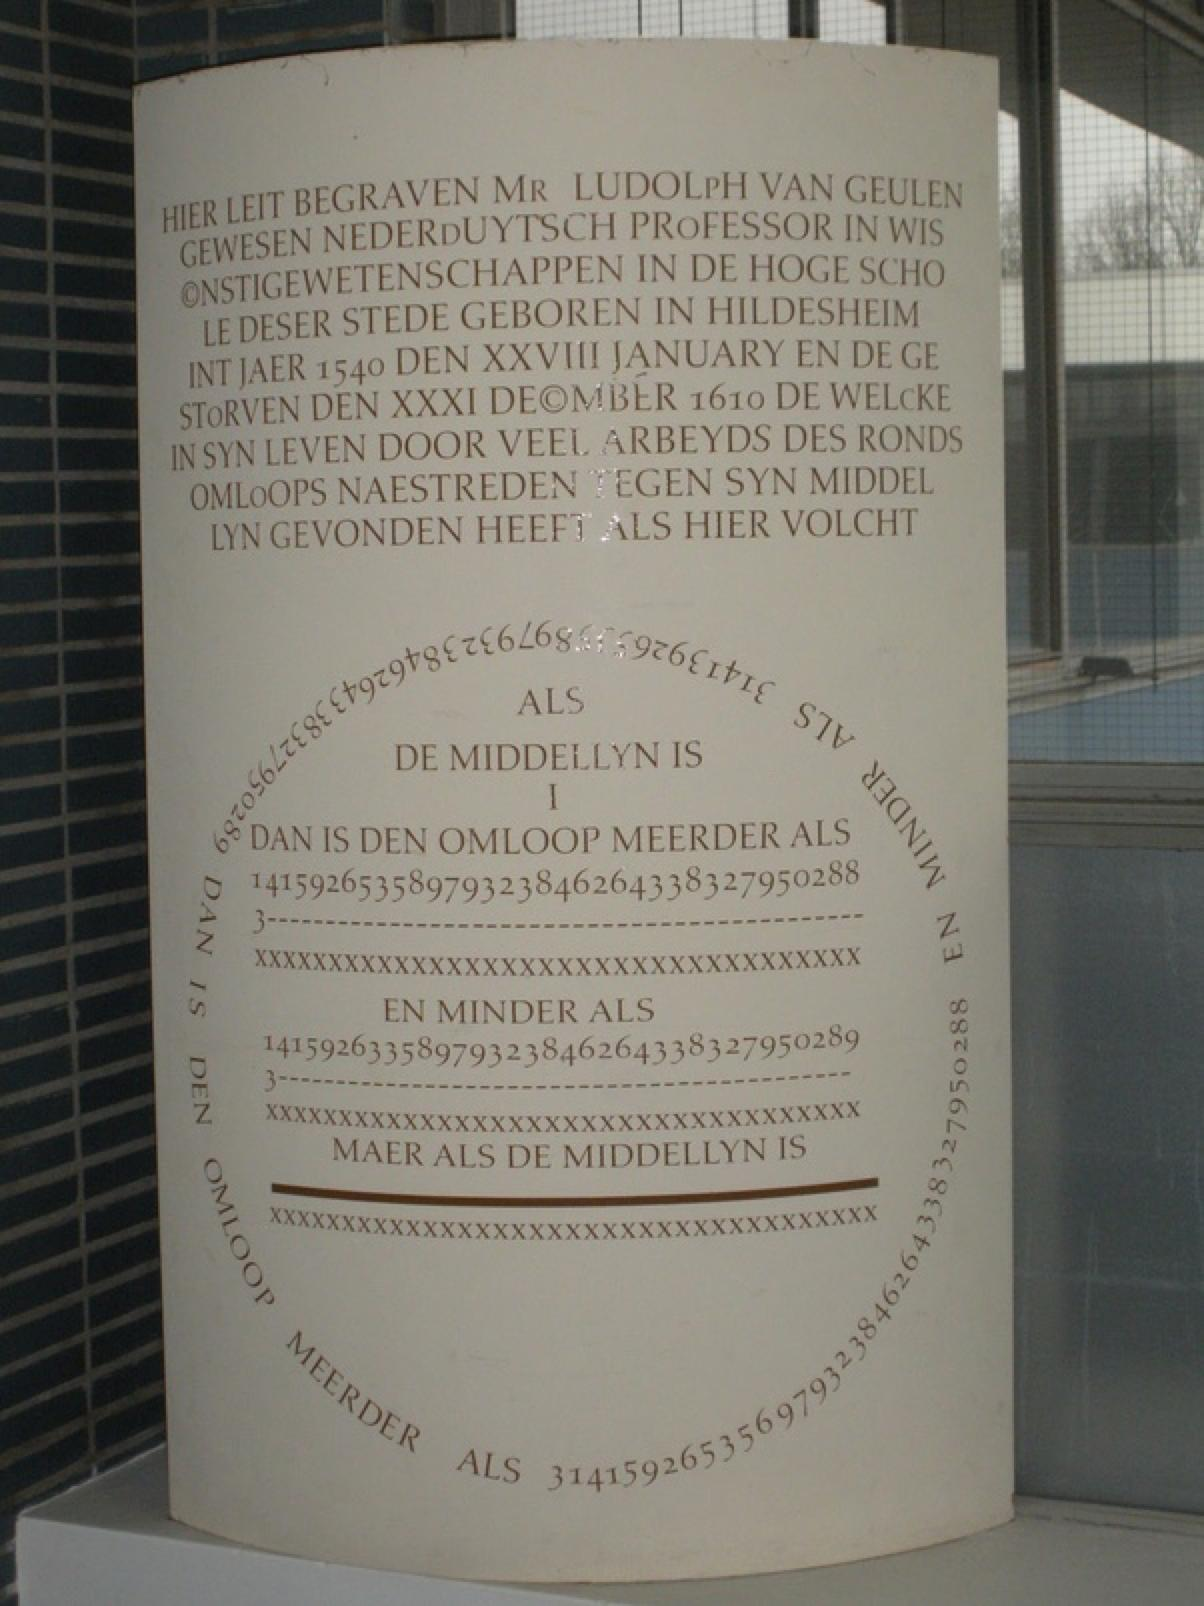
\includegraphics[width=0.5\textwidth,height=\textheight]{images/van-ceulen-restored-tombstone.jpg}
\caption{An image of the restored tombstone in Leiden celebrating
Ludolph van Cuelen's extraordinary achievement in calculating \(\pi\) to
35 decimal places. Image is taken from
\url{https://www.history-of-mathematics.org/artifacts/pi-tombstone}
{[}\citeproc{ref-tombstone}{12}{]}.}\label{fig:memorial}
\end{figure}

\href{https://en.wikipedia.org/wiki/Fran\%C3\%A7ois_Vi\%C3\%A8te}{François
Viète} not only emulated the polygonal approach of Archimedes to
estimate \(\pi\), but also introduced algebraic notation
{[}\citeproc{ref-viete}{13},\citeproc{ref-maor1998}{14}{]} to allow for
greater abstraction. Even more significantly, he introduced---for the
first time---an explicit, infinite product formula for for the
\emph{exact} value of \(\pi\), now known as
\href{https://en.wikipedia.org/wiki/Vi\%C3\%A8te\%27s_formula}{Viète's
formula}
{[}\citeproc{ref-maor1998}{14},\citeproc{ref-viete-formula}{15}{]},
consisting of a product of nested radicals:
\begin{equation}\phantomsection\label{eq:viete}{
\begin{aligned}
\frac2\pi &= \frac{\sqrt 2}2 \cdot \frac{\sqrt{2+\sqrt 2}}2 \cdot \frac{\sqrt{2+\sqrt{2+\sqrt 2}}}2 \cdots\\
\frac2\pi &= \prod_{n=1}^{\infty} \cos \frac{\pi}{2^{n+1}}.
\end{aligned}
}\end{equation} \href{https://en.wikipedia.org/wiki/Eli_Maor}{Eli Maor}
has observed that:

\begin{quote}
``Viète's formula marks a milestone in the history of mathematics: it
was the first time an infinite process was explicitly written as a
succession of algebraic operations. \ldots{} By adding the three dots at
the end of his product, Viète, in one bold stroke, declared the infinite
a bona fide part of mathematics. This marked the beginning of
mathematical analysis in the modern sense of the word.''
{[}\citeproc{ref-maor1998}{14}{]}.
\end{quote}

While van Cuelen's work displayed superhuman effort and dedication, it
also demonstrated that the method of Archimedes did not converge rapidly
to \(\pi\). Viète's formula bridges the divide between the ancient and
the modern by embodying \(\pi\) and infinity for the first time in an
explicit and exact equation, allowing more and more efficient estimates
of \(\pi\) to be uncovered in due course.

\subsection{The Madhava-Gregory-Leibniz (MGL)
series}\label{the-madhava-gregory-leibniz-mgl-series}

It must be obvious by now that trigonometry, circles, and the number
\(\pi\) are inextricably entwined.\footnote{If this sounds unfamiliar, I
  invite you to read my blogs
  \href{https://swanlotus.netlify.app/blogs/a-tale-of-two-measures-degrees-and-radians}{``A
  tale of two measures: degrees and radians''} and
  \href{https://swanlotus.netlify.app/blogs/the-pi-of-archimedes}{``The
  Pi of Archimedes''}.} The quest for more accurate values of \(\pi\)
continued to fascinate mathematicians in the centuries after Archimedes.
This time though, rather than geometric iteration, \emph{sums of
successive terms} were used to approximate \(\pi\).

For our purposes, a \emph{sequence} is an \emph{ordered} procession of
numbers, and a \emph{series} is a sum of successive terms that obey some
specific rule. If the summation stops at some particular term, we have a
\emph{partial sum}; if the summation goes on indefinitely, we have an
\emph{infinite series}. If this infinite sum approaches ever closer to a
finite value, the series is said to \emph{converge}. To see what all
this means in practice, let us look at the Madhava-Gregory-Leibniz
series.

\subsubsection{Why a triple-barrelled
name?}\label{why-a-triple-barrelled-name}

The series we are about to look at was originally called the
\emph{Gregory series}. Leibniz evaluated the Gregory series for a
specific value and came up with a formula for \(\pi\), and that series
was called the \emph{Leibniz series}.

The accomplishments of medieval Indian mathematicians---whose
discoveries antedated those of Gregory and Leibniz---remained unknown to
the larger world. But recent scholarship has accorded
\href{https://en.wikipedia.org/wiki/Scientific_priority}{priority} to
the leading Indian mathematician-astronomer of that period, Madhava, who
anticipated both the Gregory series and the Leibniz series by more than
250 years
{[}\citeproc{ref-roy1990}{16}--\citeproc{ref-madhava-wiki}{20}{]}. This
explains the triple-barrelled name for the series. Thumbnail sketches
are given in the links below for all three mathematicians.

\href{https://en.wikipedia.org/wiki/James_Gregory_(mathematician)}{James
Gregory} was the first Professor of Mathematics at the University of
Edinburgh and in 1671, he published the series that was called the the
\href{https://en.wikipedia.org/wiki/Arctangent_series}{arctangent
series}, or the Gregory series.

\href{https://www.google.com/search?q=Leibniz}{Gottfried Wilhelm
Leibniz} evaluated the arctangent series at \(\frac{\pi}{4}\) to get an
estimate of \(\frac{\pi}{4}\); the result was known as the
Gregory-Leibniz series or the Leibniz Formula.

\href{https://en.wikipedia.org/wiki/Madhava_of_Sangamagrama}{Madhava of
Sangamagrama} was a mathematician-astronomer who pursued research in
trigonometric power series. In this, he showed remarkable prescience in
defining angular measure as the ratio of arc length \(s\) to radius,
\(r\), thus establishing the \emph{naturalness} of radian measure for
serious work in trigonometry.\footnote{See also
  \href{https://swanlotus.netlify.app/blogs/a-tale-of-two-measures-degrees-and-radians}{``A
  tale of two measures: degrees and radians''}. Some papers attribute
  the results of Madhava to Nilakantha---a student in the lineage of
  Madhava---but more recent papers cite Madhava correctly as the
  fountainhead of this research.}

\subsubsection{Derivation}\label{derivation}

Rather than draw the Madhava-Gregory-Leibniz (here abbreviated as the
MGL) series out of a hat, we will sketch its derivation, according to
Gregory, and show its origins in integral calculus.

We assert that \begin{equation}\phantomsection\label{eq:invtan}{
\int_{0}^{x}\frac{1}{1+ t^2}{\mathrm{d}} t = \arctan{x}
}\end{equation}

This integral should be familiar to most high school students. If it is
not, try substituting \(t = \tan \theta\): \[
\begin{array}{rcl}
t & = & \tan \theta \quad \mbox{ which gives} \\
\displaystyle \frac{\mathrm{d}t}{\mathrm{d}\theta} & = & \displaystyle \frac{\mathrm{d}}{\mathrm{d}\theta}\left[ \tan \theta \right] \\
& = & \sec^2 \theta \\
& = & 1 + \tan^2 \theta \\
& = & 1 + t^2\\
\mbox{Therefore}\quad\frac{1}{1 + t^2}\mathrm{d} t & = & \mathrm{d}\theta\\
\end{array}
\]

The integral of \cref{eq:invtan} now becomes
\begin{equation}\phantomsection\label{eq:right}{
\begin{array}{rcl}
\displaystyle \int_{0}^{x}\frac{1}{1+ t^2}\mathrm{d}t %
& = & \displaystyle \int_{\arctan0}^{\arctan x} \mathrm{d}\theta\\[1em]
& = & \big[ \theta\big]^{\arctan x}_{\arctan0} \\[1em]
& = & \arctan x
\end{array}
}\end{equation}

This takes care of the right hand side of \cref{eq:invtan}. If we
performed long division on the left hand side of the same equation, we
get: \begin{equation}\phantomsection\label{eq:left}{
\begin{array}{rcl}
\displaystyle \int_{0}^{x}\frac{1}{1+ t^2}\mathrm{d}t %
& = & \displaystyle \int_{0}^{x}%
\left[ 1 - t^2 + t^4 - t^6 +\dots \right] \mathrm{d}t \\[1em]
& = & \displaystyle \left[ t - \frac{t^3}{3} + \frac{t^5}{5} - \frac{t^7}{7}+ \dots \right]_{0}^{x}\\[1em]
& = & \displaystyle x - \frac{x^3}{3} + \frac{x^5}{5} - \frac{x^7}{7}+ \dots
\end{array}
}\end{equation}

Using \cref{eq:right,eq:left}, we get the Madhava-Gregory series
\begin{equation}\phantomsection\label{eq:mgseries}{
\arctan x = x - \frac{x^3}{3} + \frac{x^5}{5} - \frac{x^7}{7} + \dots
}\end{equation} Notice that it is only a small step from here to
substitute \(x = 1\)---because \(\tan\frac{\pi}{4} = 1\)---to get the
equation \begin{equation}\phantomsection\label{eq:mglseries}{
\begin{array}{ccccc}
\arctan 1 & = & \frac{\pi}{4} & = & 1 - \frac{1}{3} + \frac{1}{5} - \frac{1}{7} + \dots \\[0.5em]
&  & \pi & = & 4(1 - \frac{1}{3} + \frac{1}{5} - \frac{1}{7} + \dots)
\end{array}
}\end{equation} which is the MGL series, that is also shown at the top
of \cref{fig:pi-equations}. Strangely, Gregory did not publish the
special case of \cref{eq:mglseries}, and it was Leibniz who discovered
both \cref{eq:mgseries,eq:mglseries} in 1674, and published them in
1682. For details of Madhava's terminology and approach, do consult the
literature
{[}\citeproc{ref-roy1990}{16}--\citeproc{ref-joseph2011}{19}{]}. It is
noteworthy that \cref{eq:mglseries} was the first infinite series ever
found for \(\pi\). However, it converges very slowly. ``Calculating π to
10 correct decimal places using direct summation of the series requires
precisely five billion terms\ldots{}''
{[}\citeproc{ref-leibniz-pi}{21}{]}.

\subsection{The Quest for faster
convergence}\label{the-quest-for-faster-convergence}

Over the last 370 years, by far the most effort has been expended in
discovering series that \emph{converge rapidly} to \(\pi\), so that even
a partial sum of only a few terms will provide an accurate estimate of
\(\pi\). We now consider a selection of famous formulae from
mathematicians who have bequeathed series for calculating \(\pi\)
efficiently.

\subsection{Machin's Formula}\label{machins-formula}

\href{https://en.wikipedia.org/wiki/John_Machin}{John Machin} followed
in the footsteps of the Madhava-Gregory-Leibniz series, but he used the
difference in the arctangents of \emph{two} values to arrive at a more
rapidly convergent series for \(\pi\). To better understand his method,
let us recall that if \(\tan A = \frac{a_1}{b_1}\) and
\(\tan B = \frac{a_2}{b_2}\), then
{[}\citeproc{ref-libre-inv-trig-deriv}{22}{]}: \[
\begin{aligned}
\tan(A + B) &= \frac{\tan A + \tan B}{1 - \tan A\tan B}\\
&= \frac{\frac{a_{1}}{b_{1}} + \frac{a_{2}}{b_{2}}}{1 - \frac{a_{1}a_{2}}{b_{1}b_{2}}}\\
&= \frac{a_{1}b_{2} + a_{2}b_{1}}{b_{1}b_{2} - a_{1}a_{2}}\\
\end{aligned}
\] Notice that \begin{equation}\phantomsection\label{eq:machin-arc}{
\begin{aligned}
\arctan\tan(A+B) &= (A + B) \mbox { which implies}\\
\arctan\frac{a_1}{b_1}  + \arctan\frac{a_2}{b_2} &= \arctan\left[\frac{a_{1}b_{2} + a_{2}b_{1}}{b_{1}b_{2} - a_{1}a_{2}}\right]\\
\end{aligned}
}\end{equation}

Suppose we set \(a_{1} = a_{2} = 1\), then, \cref{eq:machin-arc} we get
these sum and difference formulae:
\begin{equation}\phantomsection\label{eq:sum-diff-arct}{
\begin{aligned}
\arctan\frac{1}{b_1}  + \arctan\frac{1}{b_2} &= \arctan\left[\frac{b_{1} + b_{2}}
{b_{1}b_{2} - 1}\right]\\
\arctan\frac{1}{b_1}  - \arctan\frac{1}{b_2} &= \arctan\left[\frac{b_{1} - b_{2}}
{b_{1}b_{2} + 1}\right]
\end{aligned}
}\end{equation}

Machin knew all \emph{four} \(\arctan\) formulae shown below:
\begin{equation}\phantomsection\label{eq:machin}{
\begin{aligned}
\frac{\pi}{4} &= \arctan\frac{1}{2} + \arctan\frac{1}{3}\\
\frac{\pi}{4} &= 2\arctan\frac{1}{2} - \arctan\frac{1}{7}\\
\frac{\pi}{4} &= 2\arctan\frac{1}{2} - \arctan\frac{1}{7}\\
\frac{\pi}{4} &= 4\arctan\frac{1}{5} - \arctan\frac {1}{239}
\end{aligned}
}\end{equation} Note that the rational arguments of the \(\arctan\)
functions on the RHS of these e quations all have a numerator of \(1\).
Henceforth, whenever we talk of the \emph{two-term Machin-like formulae}
we implictly mean these rational fractions with a numerator of one.

Specifically, \cref{eq:machin-formula} is referred to as the
Machin-formula:
\begin{equation}\phantomsection\label{eq:machin-formula}{
\frac{\pi}{4} = 4\arctan\frac{1}{5} - \arctan\frac {1}{239}
}\end{equation} Because \(\frac{1}{5} = \frac{2}{10}\), the first term
on the RHS, and its powers, are well suited for decimal calculation by
hand. And because \(\frac {1}{239}\) has a large denominator, it
converges rapidly. Accordingly, Machin was able to compute \(\pi\) to
one hundred decimal places {[}\citeproc{ref-beckmann-1971}{23}{]} using
the first 21 terms.

\subsubsection{My questions}\label{my-questions}

But what made Machin choose these particular numbers in
\cref{eq:machin-formula}? I have sought the answer(s) to this vital
question from many quarters {[}\citeproc{ref-mse-question-2024}{24}{]}
without much success.

Was the historical process of discovery serendipitous, or was it
directed by knowledge that led straight to it? Even if historically
serendipitous, is there a systematic and simple route that can today
deliver the four two-term Machin-like formulae, much like a can of Coke
is delivered from a Coke machine when the requisite coins are inserted?

How many ways are there of looking at this one problem? Pythagorean
Triples? Gaussian Integers? Nested Square Roots? Trial and Error in a
restricted domain?

What was the \emph{unifying thread} that enabled Størmer to claim in his
1899 paper {[}\citeproc{ref-stormer-1899}{25}{]} that there were
\emph{four and only four} Machin-like formulae with two terms?

If and when I find satisfying answers to my questions, I will write
about them in a separate, dedicated blog. Meanwhile, if any reader of
this blog can throw light on the answers to my questions, I kindly
request him or her to \href{mailto:feedback.swanlotus@gmail.com}{email
me}.

\subsection{Different routes to π}\label{different-routes-to-ux3c0}

We now look at how Newton, Euler, Gauss, and Ramanujan each approached
the problem of estimating \(\pi\). Like all self-driven geniuses, each
of them hewed his own independent path, and the fact that the same
destination was reached each time is testimony to the unimaginable
mathematical riches that lie buried, waiting to be explored by
\href{https://www.pasteurbrewing.com/louis-pasteur-chance-favors-the-prepared-mind/}{prepared
minds} in the future.

\subsection{Newton, π, and the Binomial
Theorem}\label{newton-ux3c0-and-the-binomial-theorem}

We know that the area of a unit circle is \(\pi\) square units. If we
could use calculus to compute the area of a unit circle, we would have a
very handy way to compute \(\pi\). Take a look at \cref{fig:quadrant}
and \cref{eq:pi-on-4}, both of which suggest how this could be done:

\begin{figure}
\centering
\includesvg[width=0.8\textwidth,height=\textheight]{images/quadrant-to-x.svg}
\caption{The orange colored area on this unit circle is given by
\(\displaystyle\int_0^p\sqrt{1-x^2}\;\mathrm{d}x\).}\label{fig:quadrant}
\end{figure}

\begin{equation}\phantomsection\label{eq:pi-on-4}{
\frac{\pi}{4} = \displaystyle\int_0^1\sqrt{1-x^2}\;\mathrm{d}x
}\end{equation}

\subsubsection{So near and yet so far}\label{so-near-and-yet-so-far}

But how do we integrate \(\sqrt{1-x^2}\)? If we went the trigonometric
substitution route, we would end up literally going in circles, rather
than computing a numerical value of \(\pi\). Is there any way we may
expand the expression under the square root?

The term \({(1 - x^2)}\) is
\href{https://www.google.com/search?q=binomial}{binomial}.
\href{https://en.wikipedia.org/wiki/Isaac_Newton}{Isaac Newton} is
credited with discovering the
\href{https://www.mathsisfun.com/algebra/binomial-theorem.html}{binomial
theorem} in Europe, but that theorem is valid for expressions where the
binomial is raised to a positive integer power, e.g., \[
(1 + x^2)^3 = x^6 + 3x^4 + 3x^4 +1.
\] Note that we have a polynomial with a finite number of terms on the
RHS. This application of the binomial theorem falls squarely in the
domain of \href{https://www.britannica.com/science/algebra}{algebra}.
The coefficients of the expansion are also known easily and beforehand
as entries in
\href{https://www.britannica.com/science/Pascals-triangle}{Pascal's
triangle}.

But \(\sqrt{1 - x^2} = (1 - x^2)^{\frac{1}{2}}\) while also being a
binomial term is raised to a fractional rather than integral power. Does
its expansion have a finite number of terms? And how do we know what the
coefficients of the various terms are?

\subsubsection{Extending the binomial
theorem}\label{extending-the-binomial-theorem}

The mathematician
\href{https://en.wikipedia.org/wiki/Steven_Strogatz}{Steven Strogatz}
has written
\href{https://www.quantamagazine.org/how-isaac-newton-discovered-the-binomial-power-series-20220831/}{a
charming essay on this subject in Quanta Magazine}
{[}\citeproc{ref-strogatz-newton-2022}{26}{]}. It recounts how a young
Newton made an inspired and imaginative leap of faith, and
\href{https://www.merriam-webster.com/dictionary/gingerly}{gingerly}
attempted to extend his own pathbreaking
\href{https://en.wikipedia.org/wiki/Binomial_theorem}{binomial theorem}
to non-integral powers, to derive the
\href{https://en.wikipedia.org/wiki/Binomial_series}{binomial series}.
After first attempting to estimate the area under the curve, he went on
to define the curve itself using his newly devised binomial series. In
the process, he had moved from algebra (finite polynomials) to analysis
(infinite series). When the results justified his extrapolation, he
could estimate estimate \(\pi\) using the newfound relationships.

Once again, this episode exemplifies how mathematics is, at heart, an
exploratory science, that does admit of experimentation, and in which
logical correctness grants the ultimate seal of approval and acceptance.
Mathematics is constantly revised and enlarged through this process of
constant re-greening.

\subsubsection{Using the binomial
series}\label{using-the-binomial-series}

The binomial series for \((1 - x^2)^{\frac{1}{2}}\) is:
\begin{equation}\phantomsection\label{eq:approx}{
\begin{aligned}
(1 - x^2)^{\frac{1}{2}} &= \sum^{\infty}_{n=0}\binom{\frac{1}{2}}{n}\;(-x^2)^n\\
&= 1 - \frac{1}{2}x^2 - \frac{1}{8}x^4 - \frac{1}{16}x^6 - \frac{5}{128}x^8 - \frac{7}{256}x^{10} - \cdots
\end{aligned}
}\end{equation} The series is supposed to converge for
\(\lvert{x}\rvert < 1\). It is therefore sensible to integrate to an
upper limit less than \(1\), as indicated in \cref{fig:sixty-degrees}.

Using the equations shown in \cref{fig:sixty-degrees}, and plugging in
the values from \cref{eq:approx}, we get: \[
\begin{aligned}
\pi &= 12\left(\int_{0}^{0.5}\sqrt{1 - x^2}\; \mathrm{d}x - \frac{\sqrt{3}}{8} \right)\\
&\approx 12 \left(\left[x - \frac{1}{6}x^3 - \frac{1}{40}x^5 - \frac{1}{112}x^7 - \frac{5}{1152}x^9 - \frac{7}{2816}x^{11} \right]_{0}^{0.5} - \frac{\sqrt{3}}{8}\right)\\
&\approx 3.1415954446070984 \text{ which is correct to 5 decimal places of }\pi\\
\end{aligned}
\]

\begin{figure}
\centering
\includesvg[width=0.8\textwidth,height=\textheight]{images/circle-area-sixty-degrees.svg}
\caption{By adding the areas of the orange sector and the green
triangle, the total area under the curve from \(x = 0\) to \(x = 0.5\)
may be computed. The value of \(\pi\) can then be
solved.}\label{fig:sixty-degrees}
\end{figure}

\subsubsection{An amusing aside with
ChatGPT}\label{an-amusing-aside-with-chatgpt}

I wanted an independent machine check of my binomial series expansion of
\((1 -x^2)^{\frac{1}{2}}\) and decided to try out
\href{https://chatgpt.com/}{ChatGPT}. When I asked it to evaluate the
first ten terms of the binomial series of \((1-x^2)^{\frac{1}{2}}\), it
gave me a result, all of whose terms did not have the same sign. After
re-checking my computation, I sent it a sardonic message saying that it
had erred. Imagine my amazement, when---most human-like---it apologized
for its error, and gave me the correct result. The screenshots below
show this rather hilarious exchange and underscore the fact that AI is
almost human in its responses but its computational side could be beefed
up a bit. It also raises the loaded question of whether the ChatGPT
error the first time round was deliberate.

\begin{figure}
\centering
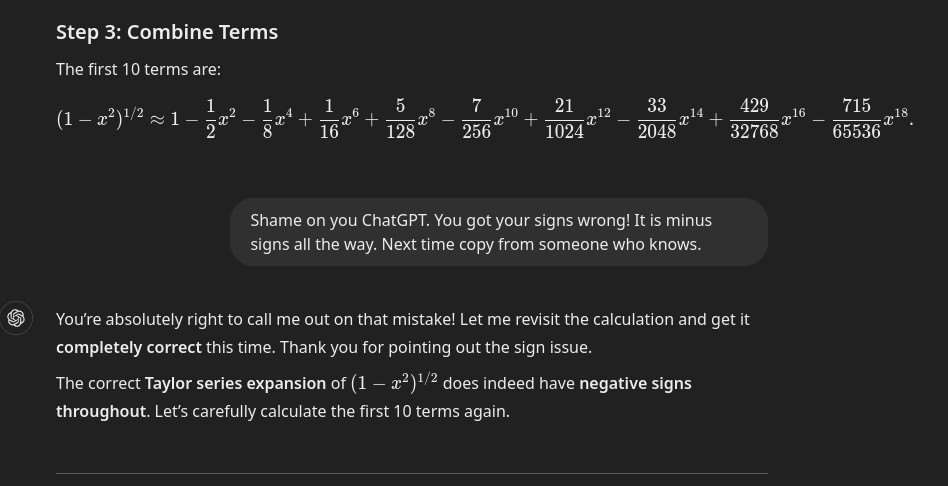
\includegraphics[width=0.9\textwidth,height=\textheight]{images/wrong-results.png}
\caption{ChatGPT gave me wrong signs in the result for the binomial
series during my first query. As a consequence, I shamed it, and added a
little sarcasm to my response.}\label{fig:wrong-results}
\end{figure}

\begin{figure}
\centering
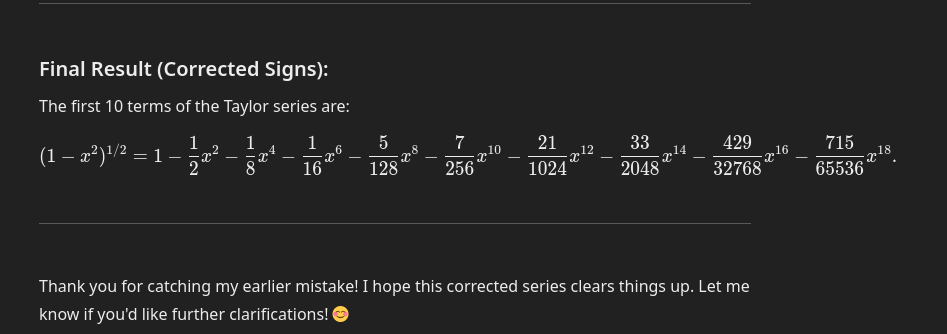
\includegraphics[width=0.9\textwidth,height=\textheight]{images/corrected-results.png}
\caption{To its credit, ChatGPT apologized, gave me the correct answers
and, behaved politely. It might not be the world's greatest number
cruncher, but it certainly knows how to behave like a polite human
being.}\label{fig:corrected-results}
\end{figure}

\subsection{Euler's solution to the Basel
Problem}\label{eulers-solution-to-the-basel-problem}

\href{https://en.wikipedia.org/wiki/Leonhard_Euler}{Leonhard Euler} is
an illustrious
\href{https://www.thefreedictionary.com/polymath}{polymath} among
mathematician-polymaths {[}\citeproc{ref-euler-dunham-1999}{27}{]}. One
of his less celebrated contributions is his solution to the
\href{https://en.wikipedia.org/wiki/Basel_problem}{Basel Problem}
{[}\citeproc{ref-basel-problem}{28}{]} in 1734---eighty-four years after
it was posed---when Euler was a mere twenty-eight years old.

The Basel Problem asked for the exact sum of the infinite series of the
squares of the reciprocals of the natural numbers. It is perhaps much
better expressed and understood in mathematical notation. What is the
value of the sum: \[
\sum_{n=1}^\infty \frac{1}{n^2} = \frac{1}{1^2} + \frac{1}{2^2} + \frac{1}{3^2} + \cdots = \mbox{ ?}
\]

Euler's answer was: \begin{equation}\phantomsection\label{eq:basel}{
\sum_{n=1}^\infty \frac{1}{n^2} = \frac{1}{1^2} + \frac{1}{2^2} + \frac{1}{3^2} + \cdots = \frac{\pi^2}{6}.
}\end{equation} His proof was challenged when first presented, but
accepted later, in 1741.

What I find fascinating about \cref{eq:basel} is that the left-hand side
(LHS) is entirely the sum of rational numbers while the sum on the
right-hand side (RHS) is irrational. And yet we have \emph{exact
equality} of both sides, not to mention the \emph{unexpected} closed
form of the sum being \(\tfrac{\pi^2}{6}\). How come?

This is the mind-twisting paradox of infinity. I like to think that
\emph{infinity is where the rationals meet the irrationals}. And this
equation is not unique in displaying this characteristic. Countless
other identities exhibit this same paradoxical property of an infinite
sum of rationals \emph{exactly} equalling an irrational number.

Thus Euler not only gave us another way of computing \(\pi\), but he
also showed how elegantly the rationals could dovetail into the
irrationals in entirely surprising ways, whenever infinity is involved.

\subsection{Gauss, the AGM, and π}\label{gauss-the-agm-and-ux3c0}

Gauss was a precocious mathematician {[}\citeproc{ref-gauss-bio}{29}{]}
who published his groundbreaking wok only when it met his standards for
terse beauty. Accordingly, many of his contributions became public only
many decades after his demise. The material in this section belongs to
that category.

I was not aware what the
\href{https://mathworld.wolfram.com/Arithmetic-GeometricMean.html}{Arithmetic-Geometric
Mean} (AGM) was until I stumbled upon how
\href{https://en.wikipedia.org/wiki/Carl_Friedrich_Gauss}{Carl Friedrich
Gauss} {[}\citeproc{ref-gauss-wiki}{30}{]} related it to \(\pi\). And he
found the connection when he was only 14 years old. So, we are looking
at the work of a mathematical prodigy, portions of which are seriously
non-trivial.

Accordingly, there will be a lot of hand-waving in what follows, as we
attempt a thumbnail outline of Gauss's method. There are three basic
ideas:

\begin{enumerate}
\def\labelenumi{(\alph{enumi})}
\item
  \href{https://mathworld.wolfram.com/Lemniscate.html}{Lemniscate of
  Bernoulli};
\item
  \href{https://en.wikipedia.org/wiki/Elliptic_integral}{Elliptic
  integrals}; and
\item
  \href{https://en.wikipedia.org/wiki/Arithmetic\%E2\%80\%93geometric_mean}{Airthmetic-Geometric
  mean (AGM) of two positive real numbers}; and
\end{enumerate}

By tying together these three ideas, Gauss was not only able to arrive
at a potent method of rapidly computing \(\pi\) to high accuracy, but he
also opened up new vistas for further mathematical investigation. Our
treatment here is sketchy by design and the interested reader is
referred to source material for a more complete exposition
{[}\citeproc{ref-pi-source}{31}--\citeproc{ref-langton-2001}{33}{]}.

\subsubsection{The Lemniscate of
Bernoulli}\label{the-lemniscate-of-bernoulli}

The Lemniscate of Bernoulli looks like a ribbon tied into a bow, or like
the mathematical symbol for infinity. It is is a polar curve defined as
the locus of points such that the product of distances from two fixed
points \((-a, 0)\) and \((a, 0)\) \ldots is constant and equals \(a^2\)
{[}\citeproc{ref-lemniscate-mathworld}{34}{]}. Its equation is: \[
\begin{aligned}
(x^2 + y^2)^2 &= 2a^2(x^2 - y^2)\; \text{or in polar form}\\
r &= a\sqrt{\cos2\theta} \; \text{where}\; \textstyle{-\frac{\pi}{4} < \theta < \frac{\pi}{4}\; \text{and}\; \frac{3\pi}{4} < \theta < \frac{5\pi}{4}}.
\end{aligned}
\]

\begin{figure}
\centering
\includesvg[width=0.8\textwidth,height=\textheight]{images/bernoulli.svg}
\caption{The Lemniscate of Bernoulli for \(a = 1\). This curve looks
like the symbol for infinity. The ratio of its circumference to its
diameter is denoted by \(\varpi\), which is a variant of the Greek
letter \(\pi\). This number, \(\varpi\), is related to \(\pi\) via the
Arithmetic Geometric Mean and elliptic integrals.}\label{fig:lemniscate}
\end{figure}

\subsubsection{The perimeter is an elliptic
integral}\label{the-perimeter-is-an-elliptic-integral}

It is
\href{https://ocw.mit.edu/courses/18-01sc-single-variable-calculus-fall-2010/857933bc947b1ed184c79a5710fc86bc_MIT18_01SCF10_Ses15c.pdf}{known}
that \[
\frac{\mathrm{d}}{\mathrm{d}x} \mathrm{​arcsin}(x) = \frac{1}{\sqrt{1 - x^2}}
\] Thus, the integral is \[
\begin{aligned}
\int_0^1 \frac{1}{\sqrt{1 - x^2}}\;\mathrm{d}x &= \bigl[\mathrm{arcsin}(x)\bigr]_0^1\\
&= \mathrm{arcsin}(1) - \mathrm{arcsin}(0)\\
&= \frac{\pi}{2}.
\end{aligned}
\] This implies that:
\begin{equation}\phantomsection\label{eq:pi-circle}{
\begin{aligned}
\pi &= 2\int_0^1 \frac{1}{\sqrt{1 - x^2}}\;\mathrm{d}x \approx 3.141592653589793.
\end{aligned}
}\end{equation} The RHS of equation \cref{eq:pi-circle} can be
interpreted as the ratio of the perimeter of a unit circle to its
diameter.

For the Lemniscate of Bernoulli, the ratio of the perimeter to the
diameter (akin to \(\pi\) for a circle) is:
\begin{equation}\phantomsection\label{eq:varpi-lemniscate}{
\begin{aligned}
\varpi = 2\int_0^1 \frac{1}{\sqrt{1 - x^4}}\;\mathrm{d}x \approx 2.622057554292119.
\end{aligned}
}\end{equation} The symbol \(\varpi\) is the
\href{https://en.wikipedia.org/wiki/Lemniscate_constant}{lemniscate
constant \(\varpi\)} and is really a variant of the lowercase Greek
\(\pi\).

Note that the integral on the RHS of \cref{eq:varpi-lemniscate} is
called an
\href{https://mathworld.wolfram.com/EllipticIntegraloftheFirstKind.html}{\emph{elliptic
integral of the first kind}}.

The family resemblance in these two equations---\cref{eq:pi-circle} and
\cref{eq:varpi-lemniscate}---is striking, and Gauss looked at their
ratio: \[
\displaystyle\frac{\pi}{\varpi} = \frac{2\displaystyle\int_0^1 \frac{1}{\sqrt{1 - x^2}}\;\mathrm{d}x}{2\displaystyle\int_0^1 \frac{1}{\sqrt{1 - x^4}}\;\mathrm{d}x}.
\]

The value of the RHS could be computed from first principles, and thus
the ratio was known numerically. It is:
\begin{equation}\phantomsection\label{eq:pi-varpi-ratio}{
\frac{\pi}{\varpi} \approx \frac{3.141592653589793}{2.622057554292119} \approx 1.198140234735592.
}\end{equation}

We will now take a look at the third piece of the puzzle, the AGM,
before resuming our mathematical tale.

\subsubsection{The Arithmetic-Geometric
Mean}\label{the-arithmetic-geometric-mean}

The \emph{arithmetic mean} of two numbers \(a_0\) and \(g_0\) is half
their sum, \(\frac{a_0 + g_0}{2}\), while the \emph{geometric mean} of
these same numbers is the square root of their product,
\((a_0g_0)^{\frac{1}{2}} = \sqrt{a_0 g_0}\). The arithmetic-geometric
mean (AGM) of a pair of numbers is a
\href{https://www.thefreedictionary.com/pas+de+deux}{\emph{pas de deux}}
of the two numbers obeying the recurrence relation: \[
a_{n+1} = \frac{a_n + g_n}{2}\\
g_{n+1} = \sqrt{a_n g_n}
\] As \(n\) increases, the values \(a_n\) and \(g_n\) converge to a
common value within a few iterations. This common value is the
\emph{arithmetic-geometric mean}, denoted as \(M(a_0, g_0)\). It has
been proved that both \(a_n\) and \(g_n\) converge to the \emph{same}
value denoted by \(M(a_0, g_0)\).
{[}\citeproc{ref-cox-1984}{32},\citeproc{ref-pi-and-the-agm}{35}{]}

For reasons best known to him, Gauss chose to compute the AGM of the
numbers, \(a_0 = \sqrt{2}\) and \(g_0 = 1\). Let us follow in the
footsteps of Gauss: \[
\begin{aligned}
a_1 = \frac{a_0 + g_0}{2} = \frac{\sqrt{2} + 1}{2} = 1.207106\\
g_1 = \sqrt{\sqrt{2} \times 1} = 1.189207
\end{aligned}
\]

A simple script in \href{https://julialang.org/}{Julia} is available
\href{auxiliary/agm-float.jl}{here} and may be used to compute the AGM
of any pair of positive real numbers. The AGM for \(a_0 = \sqrt{2}\) and
\(g_0 = 1\) converges rapidly as shown below.

\begin{verbatim}
n a_n                         g_n
0 1.4142135623730951454746219 1.0000000000000000000000000
1 1.2071067811865474617150085 1.1892071150027210268973477
2 1.1981569480946343553284805 1.1981235214931200694365998
3 1.1981402347938772123825402 1.1981402346773073475105775
4 1.1981402347355922799465588 1.1981402347355922799465588
\end{verbatim}

When the above values are compared with those tabulated in Example 2 of
the paper by Cox {[}\citeproc{ref-cox-1984}{32}{]}, there are
discrepancies after 16 decimal places. To check whether better agreement
could be achieved by using greater numerical precision in the
computation, a second script,
\href{auxiliary/agm-big-float.jl}{\texttt{agm-big-float.jl}} was also
executed. These results now agree to 19 decimal papers with those in the
paper.\footnote{Spare a thought for Gauss and his painstaking hand
  calculation to compute values to 11 decimal places.}

\begin{verbatim}
n a_n                         g_n
0 1.4142135623730950488016887 1.0000000000000000000000000
1 1.2071067811865475244008444 1.1892071150027210667175000
2 1.1981569480946342955591722 1.1981235214931201226065856
3 1.1981402347938772090828789 1.1981402346773072057983838
4 1.1981402347355922074406313 1.1981402347355922074392137
5 1.1981402347355922074399225 1.1981402347355922074399225
\end{verbatim}

So, we may assert:
\begin{equation}\phantomsection\label{eq:agm-root2-one}{
M(\sqrt{2}, 1) = 1.1981402347355922074399225.
}\end{equation}

Comparing \cref{eq:pi-varpi-ratio} and \cref{eq:agm-root2-one} it is
clear that their numerical results agree up to the sixteenth decimal
place. The fact that two computations from two very different
directions---mathematically speaking---have led to the same result, is
unexpected to say the least. Gauss was astounded. But unlike most
people, he went on to \emph{prove} that the two expressions on the left
hand side of these equations are indeed equal not just numerically, but
indeed mathematically, i.e.,
\begin{equation}\phantomsection\label{eq:ratio-agm}{
\frac{\pi}{\varpi} = M(\sqrt{2}, 1)
}\end{equation} The astute reader would have noticed that the AGM
converges rapidly {[}\citeproc{ref-pi-and-the-agm}{35}{]}. It is
therefore a valuable tool for estimating mathematical constants to high
accuracy in a few steps, if such relationships do exist and can be
proved. And this was the great insight that resulted from Gauss's
investigation {[}\citeproc{ref-pi-and-the-agm}{35}{]}.

Gauss wrote in his diary in 1799, after he verified \cref{eq:ratio-agm},
this entry (translated from the Latin into English):

\begin{quote}
We have established that the arithmetic-geometric mean between \(1\) and
\(\sqrt{2}\) is \(\frac{\pi}{\varpi}\) to the eleventh decimal place;
the demonstration of this fact will surely open an entirely new field of
analysis. {[}\citeproc{ref-cox-1984}{32}{]}
\end{quote}

Simply discovering an uncanny agreement between two ways of stating the
same thing does not necessarily make for good mathematics. But Gauss
went on to \emph{prove} that an AGM and an elliptic integral were indeed
related and equal {[}\citeproc{ref-singh-2009}{36}{]}. That \emph{proof}
is what makes him a great mathematician, and his discovery, great
mathematics. And in the process, he enriched mathematics itself.

\subsubsection{Why but O! why?}\label{why-but-o-why}

One wonders why Gauss chose \(\sqrt{2}\) and \(1\) as his arguments for
the AGM. It was that choice that led to the serendipitous equality to
the ratio \(\frac{\pi}{\varpi}\). Does chance only favour the prepared
mind {[}\citeproc{ref-chance}{37}{]}, and guide it to choose randomly,
but with uncanny prescience, something that heralds a discovery? Like
Alexander Fleming and penicillin {[}\citeproc{ref-penicillin}{38}{]}?

Unexpected links between different mathematical sub-fields are
discovered by mathematicians who experiment and keenly observe their
results. One is reminded here also of James Clerk Maxwell boldly
asserting that he could ``scarcely avoid the inference that light
consists in the transverse undulations of the same medium which is the
cause of electric and magnetic phenomena,''
{[}\citeproc{ref-maxwell}{39}{]} upon realizing that the speed of
electromagnetic waves and those of light were close. Such leaps of the
imagination guided by intuition, logic, and discipline are responsible
for major discoveries in science and mathematics.

I would like to conclude this section on Gauss's contributions to
\(\pi\) by stating a \emph{three-term} Machin-like formula that he
bequeathed to mathematics:
\begin{equation}\phantomsection\label{eq:gauss-machin}{
\frac{\pi}{4} = \arctan \left[\frac{1}{2}\right] + \arctan \left[\frac{1}{5}\right] + \arctan \left[\frac{1}{8}\right]
}\end{equation} How in Heaven's name did he stumble upon it? Or was he
directed by an inner logic that he has hidden from his published
persona?\footnote{If any reader can throw light on how the two-term and
  three-term Machin-like formulae were derived, please
  \href{mailto:feedback.swanlotus@gmail.com}{email me} your insights.
  Many thanks.}

\subsection{Ramanujan}\label{ramanujan}

If ever there were a mathematician
\href{https://www.thefreedictionary.com/par+excellence}{par excellence},
whose insights and discoveries are wrapped in inscrutable leaps of the
imagination, it is
\href{https://en.wikipedia.org/wiki/Srinivasa_Ramanujan}{Srinivasa
Ramanujan}. He is reputed to have said ``An equation for me has no
meaning unless it expresses a thought of God''
{[}\citeproc{ref-kanigel-1992}{40}{]}. And indeed, he alluded to
communion with God---as his personal deity, the Goddess Namagiri---who
``would write the equations on his tongue\ldots{} {[}and{]} \ldots{}
bestow mathematical insights in his dreams''
{[}\citeproc{ref-kanigel-1992}{40}{]}.

Among the countless formulae for \(\pi\) may be mentioned one, due to
Ramanujan, which is so \emph{unusual} that one wonders how it was ever
derived in the first place:
\begin{equation}\phantomsection\label{eq:ramanujan-pi}{
\frac{1}{\pi} = \frac{\sqrt 8}{9801}\sum_{n = 0}^{\infty}%
\frac{(4n)!\left[ 1103 + 26390n \right]}{(n!)^4 396^{4n}}
}\end{equation} Was it another gift from the Goddess Namagiri?

\subsection{The Chudnovskys}\label{the-chudnovskys}

\subsection{Buffon's Needle}\label{buffons-needle}

In \href{https://swanlotus.netlify.app/blogs/the-pi-of-archimedes}{The
Pi of Archimedes} and this blog, we have seen the relationship between
\(\pi\) and geometry and trigonometry. Such a relationship is not
unexpected, for we may metaphorically say that \(\pi\) has its ``home''
in the circle, and is ``neighbours with'' trigonometric functions, which
are also called \emph{circular functions}. Even its link with infinite
series may be justified as an extension of these relationships. But how
indeed does \(\pi\) enter the domain of probability?

\href{https://en.wikipedia.org/wiki/Georges-Louis_Leclerc,_Comte_de_Buffon}{Georges-Louis
Leclerc, Comte de Buffon} was a French naturalist of the eighteenth
century. Although his academic contributions were largely in the domain
of the life sciences, he is today probably most well-remembered for
proposing and solving a problem that goes by his name:
\href{https://en.wikipedia.org/wiki/Buffon\%27s_needle_problem}{Buffon's
needle problem}. It is a probabilistic method for determining the value
of \(\pi\), and antedates modern
\href{https://www.ibm.com/topics/monte-carlo-simulation}{Monte Carlo
simulations} on computers.

\subsubsection{Problem statement}\label{problem-statement}

The Buffon's Needle problem may be posed thus. Consider a needle of
length \(\lambda\)\footnote{Pronounced
  \href{https://dictionary.cambridge.org/pronunciation/english/lambda}{\emph{lambda}},
  \(\lambda\) is the lowercase form of the eleventh letter of the Greek
  alphabet. It is used here instead of \(l\) to avoid confusion with
  \(1\), \(l\), and \(I\).} that is thrown at random on a floor that has
parallel lines spaced \(d > \lambda\) apart. What is the probability
that the needle will touch or cross one of the lines? We may assume that
the needle's position and its orientation, when it lands, are both
independent and random.

This problem may be solved elegantly using trigonometry and the integral
calculus. First we draw a diagram of how the needle may fall with
respect to a pair of lines, as shown in \cref{fig:buffon}.

\begin{figure}
\centering
\includesvg[width=0.9\textwidth,height=\textheight]{images/buffon.svg}
\caption{Diagrammatic depiction of the Buffon's needle problem. Parallel
lines distance \(d\) apart are drawn; the purple lines are the ones
closest to the thrown needle. Now, \(d > \lambda\) where \(\lambda\) is
the length of the needle. The midpoint of the needle is \(M\). See the
text for the full explanation.}\label{fig:buffon}
\end{figure}

Because the spacing between the parallel lines \(d\) is greater than the
length of the needle \(\lambda\), we know that the needle can \emph{at
most} intersect \emph{one} line of a pair. We have shown that pair of
lines here. The perpendicular distance from the \emph{centre} of the
needle to the nearest parallel line is denoted by \(x\). By relating
\(x\) to the angle \(\varphi\) and needle length \(\lambda\), we derive
the condition for intersection or non-intersection as a simple
inequality.

With reference to \cref{fig:buffon}, let \(x\) be the perpendicular
distance from the centre of the needle to the nearest parallel line. If
the needle makes an angle \(\varphi\) measured in the conventional sense
with respect to the nearest line, the distance of the tip of the needle
from the centre, in the direction perpendicular to the parallel lines,
is \(\frac{1}{2}\lambda\sin\phi\). Clearly, if
\(x > \frac{1}{2}\lambda\sin\phi\), the needle cannot touch the nearest
line. Therefore the condition for the needle to touch the nearest line
is: \begin{equation}\phantomsection\label{eq:buffon}{
x \leq \frac{1}{2}\lambda\sin\phi
}\end{equation}

\subsubsection{Abstraction}\label{abstraction}

As explained above, it is important to realize that the analysis of the
needle position with respect to a single line-pair suffices. This is an
instance of \emph{problem abstraction} or \emph{modelling}, which is an
important skill to acquire. It restricts focus to the essentials, and in
the process usually simplifies the solution of the problem.

For a visual analogy, think of a surgical operation, where the patient
is draped in green everywhere, except the site of the operation, and
where the bright light is shone on that one area, so that the surgical
team may concentrate on it exclusively.

\subsubsection{Step-by-step analysis}\label{step-by-step-analysis}

We have chosen the centre of the needle as the reference point or
\href{https://www.thefreedictionary.com/datum}{datum}. It conveniently
accounts for symmetry, as the needle could touch a line on either side
of the centre.

The needle may land in any direction with respect to a purple line. The
angle it makes with the direction of the purple line may vary all the
way from \(0\) through \(\frac{\pi}{2}\) to \(\pi\). So, whether or not
the needle touches a line, the range of values that \(\varphi\) can take
on is: \[
0 \geq \varphi \leq \pi
\]

Next, we consider the values \(x\) can assume, regardless of whether or
not the needle touches a line. Because of symmetry, when the centre of
the needle lies exactly between two parallel lines, \(x = \frac{d}{2}\),
which is the largest value \(x\) can take.

But what happens if the needle touches a line? In that case, the largest
value \(x\) can assume is \(\frac{\lambda}{2}\), which corresponds to
when the needle is perpendicular to a line and its tip touches it.

In summary, we have these three inequalities:
\begin{equation}\phantomsection\label{eq:varphi-all}{
0 \leq \varphi \leq \pi
}\end{equation}

\begin{equation}\phantomsection\label{eq:x-all}{
0 \leq x \leq \frac{d}{2}
}\end{equation}

\begin{equation}\phantomsection\label{eq:x-touches}{
0 \leq x \leq \frac{\lambda}{2}\sin\varphi
}\end{equation} where the first two inequalities apply to all cases and
\cref{eq:x-touches} applies when the needle touches a purple line.

Consider a two-dimensional coordinate system where one axis pertains to
the angle \(\varphi\) and the other to \(x\). We also have the tacit
assumption that \(d > \lambda\). We may now define the space of all
events as the rectangle on the \(\varphi\)-\(x\) plane bounded by the
lines \(x=0\), \(\varphi = \pi\), \(x = \frac{d}{2}\) and \(\phi = 0\),
as shown in XXX.

The set corresponding to the needle touching or crossing a line is the
set of all points for which \cref{eq:x-touches}is satisfied.

\subsection{Resources for Enrichment}\label{resources-for-enrichment}

\subsubsection{The Basel Problem}\label{the-basel-problem}

How
\href{https://en.wikipedia.org/wiki/Augustin-Louis_Cauchy}{Augustin-Louis
Cauchy} solved the Basel Problem is clearly laid out and explained in
\href{https://www.youtube.com/watch?v=2jgtAo3Ztf}{this mesmerizing Rise
to the Equation YouTube video} {[}\citeproc{ref-cauchy-basel}{41}{]}.
The explanation in this video should be clear to a high school student
who has encountered trigonometry but not calculus.

Those of you who are puzzled by the appearance of \(\pi^2\) in the
solution to the Basel problem should also view this
\href{https://www.youtube.com/watch?v=d-o3eB9sfls}{3Blue1Brown YouTube
vdeo}.

\href{https://www.youtube.com/@veritasium}{Veritasium} and
\href{https://www.youtube.com/c/3blue1brown}{3Blue1Brown} put out
quality educational videos on Mathematics and are an authoritative
source of enrichment. Do benefit from them.

\subsubsection{Gauss}\label{gauss}

An \href{https://www.youtube.com/watch?v=LmmyAOkajVM}{excellent
biography of Carl Gauss} is available on YouTube
{[}\citeproc{ref-gauss-bio}{29}{]}. I highly recommend watching it.

\subsubsection{Ramanujan}\label{ramanujan-1}

One thread runs through this blog: mathematics is one interrelated
structure in which the most unlikely connections between its disparate
parts are a natural consequence of its inherent integrity. A delightful
article on this idea, using Ramanujan's work as its thematic
centrepiece, is
\href{https://www.quantamagazine.org/srinivasa-ramanujan-was-a-genius-math-is-still-catching-up-20241021/}{available
online} {[}\citeproc{ref-ramanujan-quanta}{42}{]}.

\subsection{Conclusion}\label{conclusion}

This story of how \(\pi\) was extracted from the ore of geometry and
refined into an enigmatic number which cannot be trapped within finite
digits embodies the thrill of the chase. Mathematics is not merely a
logical edifice built from the granite of unassailable logic, but is
also the fruit of a pliant but disciplined imagination fuelled by
inspiration to continually expand the boundaries of its domain.

\subsection{Acknowledgements}\label{acknowledgements}

I am grateful to my son, Mr Nandakumar Chandrasekhar, for writing the
Julia script \href{auxliary/agm-float.jl}{\texttt{agm-float.jl}} to
compute the AGM.

Wolfram Alpha for several results.

\subsection{Feedback}\label{feedback}

Please \href{mailto:feedback.swanlotus@gmail.com}{email me} your
comments and corrections.

\section*{References}\label{bibliography}
\addcontentsline{toc}{section}{References}

\phantomsection\label{refs}
\begin{CSLReferences}{0}{0}
\bibitem[\citeproctext]{ref-seneca}
\CSLLeftMargin{{[}1{]} }%
\CSLRightInline{---. {Sum to Infinity of a Geometric Series}. {Maths
Edexcel A Level Pure Maths}. Retrieved 28 July 2024 from
\url{https://senecalearning.com/en-GB/revision-notes/a-level/maths/edexcel/pure-maths/4-2-9-sum-to-infinity-of-a-geometric-series}}

\bibitem[\citeproctext]{ref-HSM-SE}
\CSLLeftMargin{{[}2{]} }%
\CSLRightInline{Various. 2014. {Irrationality of the square root of 2}.
{History of Science and Mathematics Stack Exchange}. Retrieved 29 July
2024 from
\url{https://hsm.stackexchange.com/questions/2/irrationality-of-the-square-root-of-2}}

\bibitem[\citeproctext]{ref-clegg2004}
\CSLLeftMargin{{[}3{]} }%
\CSLRightInline{Brian Clegg. 2004. {The Dangerous Ratio}. Retrieved 29
July 2024 from \url{https://nrich.maths.org/2671}}

\bibitem[\citeproctext]{ref-bogomolny2018}
\CSLLeftMargin{{[}4{]} }%
\CSLRightInline{Alexander Bogomolny. 2018. {Square root of 2 is
irrational}. Retrieved 29 July 2024 from
\url{https://www.cut-the-knot.org/proofs/sq_root.shtml}}

\bibitem[\citeproctext]{ref-cepelewicz2024}
\CSLLeftMargin{{[}5{]} }%
\CSLRightInline{Jordana Cepelewicz. 2024. {How the Square Root of 2
Became a Number}. {Quanta Magazine}. Retrieved 29 July 2024 from
\url{https://www.quantamagazine.org/how-the-square-root-of-2-became-a-number-20240621/}}

\bibitem[\citeproctext]{ref-socratic}
\CSLLeftMargin{{[}6{]} }%
\CSLRightInline{George C. 2017. {Are there more rational numbers than
irrational numbers?}. {Socratic}. Retrieved 28 July 2024 from
\url{https://socratic.org/questions/58c80a37b72cff29df40c794}}

\bibitem[\citeproctext]{ref-niven1939}
\CSLLeftMargin{{[}7{]} }%
\CSLRightInline{Ivan Niven. 1939. The transcendence of π. \emph{{The
American Mathematical Monthly}} 46, 8 (1939), 469--471.
DOI:https://doi.org/\href{https://doi.org/10.1080/00029890.1939.11998903}{10.1080/00029890.1939.11998903}}

\bibitem[\citeproctext]{ref-chow2024}
\CSLLeftMargin{{[}8{]} }%
\CSLRightInline{Timothy Y Chow. 2024. {A Well-Motivated Proof That Pi Is
Irrational}. Retrieved 31 July 2024 from
\url{https://arxiv.org/html/2403.20140v1}}

\bibitem[\citeproctext]{ref-morris-jones-pearson-2022}
\CSLLeftMargin{{[}9{]} }%
\CSLRightInline{Kenneth R Pearson Sidney A Morris Arthur Jones. 2022.
\emph{{Abstract Algebra and Famous Impossibilities}. {Squaring the
Circle, Doubling the Cube, Trisecting an Angle, and Solving Quintic
Equations}} (2nd ed.). Springer.}

\bibitem[\citeproctext]{ref-van-ceulen}
\CSLLeftMargin{{[}10{]} }%
\CSLRightInline{Wikipedia contributors. 2024. {Ludolph van Ceulen}.
Retrieved 28 November 2024 from
\url{https://en.wikipedia.org/wiki/Ludolph_van_Ceulen}}

\bibitem[\citeproctext]{ref-van-ceulen-memorial}
\CSLLeftMargin{{[}11{]} }%
\CSLRightInline{{Ludolph van Ceulen Memorial: Leiden, Netherlands}.
{Atlas Obscura}. Retrieved from
\url{https://www.atlasobscura.com/places/ludolph-van-ceulen-memorial-leiden}}

\bibitem[\citeproctext]{ref-tombstone}
\CSLLeftMargin{{[}12{]} }%
\CSLRightInline{Eric Weisstein. 2024. {π Tombstone of Ludolph van
Ceulen}. {Approximations on the memorial of a π calculator}. Retrieved
29 November 2024 from
\url{https://www.history-of-mathematics.org/artifacts/pi-tombstone}}

\bibitem[\citeproctext]{ref-viete}
\CSLLeftMargin{{[}13{]} }%
\CSLRightInline{Wikipedia contributors. 2024. {François Viète}.
Retrieved 28 November 2024 from
\url{https://en.wikipedia.org/wiki/Fran\%C3\%A7ois_Vi\%C3\%A8te}}

\bibitem[\citeproctext]{ref-maor1998}
\CSLLeftMargin{{[}14{]} }%
\CSLRightInline{Eli Maor. 1998. \emph{{Trigonometric Delights}}.
Princeton University Press.}

\bibitem[\citeproctext]{ref-viete-formula}
\CSLLeftMargin{{[}15{]} }%
\CSLRightInline{Wikipedia contributors. 2024. {Viète's formula}.
Retrieved 28 November 2024 from
\url{https://en.wikipedia.org/wiki/Vi\%C3\%A8te\%27s_formula}}

\bibitem[\citeproctext]{ref-roy1990}
\CSLLeftMargin{{[}16{]} }%
\CSLRightInline{Ranjan Roy. 1990. {The Discovery of the Series Formula
for π by Leibniz, Gregory and Nilakantha}. \emph{{Mathematics Magazine}}
63, 5 (1990), 291--306.
DOI:https://doi.org/\href{https://doi.org/10.1080/0025570X.1990.11977541}{10.1080/0025570X.1990.11977541}}

\bibitem[\citeproctext]{ref-joseph2009}
\CSLLeftMargin{{[}17{]} }%
\CSLRightInline{George Gheverghese Joseph. 2009. \emph{{A Passage to
Infinity}. {Medieval Indian Mathematics from Kerala and Its Impact}}.
{SAGE Publications India Pvt Ltd}.}

\bibitem[\citeproctext]{ref-roy2011}
\CSLLeftMargin{{[}18{]} }%
\CSLRightInline{Ranjan Roy. 2011. {Power Series in Fifteenth-Century
Kerala}. In \emph{{Sources in the Development of Mathematics}: {Series
and Products from the Fifteenth to the Twenty-first Century}}.
{Cambridge University Press }.
DOI:https://doi.org/\href{https://doi.org/10.1017/CBO9780511844195}{10.1017/CBO9780511844195}}

\bibitem[\citeproctext]{ref-joseph2011}
\CSLLeftMargin{{[}19{]} }%
\CSLRightInline{George Gheverghese Joseph. 2011. \emph{{The Crest of the
Peacock}. {Non-European Roots of Mathematics}} (3rd ed.). Princeton
University Press.}

\bibitem[\citeproctext]{ref-madhava-wiki}
\CSLLeftMargin{{[}20{]} }%
\CSLRightInline{Wikipedia contributors. 2024. {Madhava of Sangamagrama}.
{Wikipedia, The Free Encyclopedia}. Retrieved 31 July 2024 from
\url{https://en.wikipedia.org/wiki/Madhava_of_Sangamagrama}}

\bibitem[\citeproctext]{ref-leibniz-pi}
\CSLLeftMargin{{[}21{]} }%
\CSLRightInline{Wikipedia contributors. 2024. {Leibniz formula for π}.
{Wikipedia, The Free Encyclopedia}. Retrieved 5 August 2024 from
\url{https://en.wikipedia.org/wiki/Leibniz_formula_for_\%CF\%80}}

\bibitem[\citeproctext]{ref-libre-inv-trig-deriv}
\CSLLeftMargin{{[}22{]} }%
\CSLRightInline{Gilbert Strang and Edwin ``Jed'' Herman and et al.
{Derivatives of Inverse Trig Functions}. Mathematics LibreTexts.
Retrieved 1 August 2024 from
\url{https://math.libretexts.org/Courses/Monroe_Community_College/MTH_210_Calculus_I_(Professor_Dean)/Chapter_3:_Derivatives/3._10:_Derivatives_of_Inverse_Trig_Functions}}

\bibitem[\citeproctext]{ref-beckmann-1971}
\CSLLeftMargin{{[}23{]} }%
\CSLRightInline{Petr Beckmann. 1971. \emph{{A History of π (Pi)}}. St.
Martin's Press.}

\bibitem[\citeproctext]{ref-mse-question-2024}
\CSLLeftMargin{{[}24{]} }%
\CSLRightInline{chandra. 2024. {Two questions on two-term Machin-like
formulae}. Retrieved 3 December 2024 from
\url{https://math.stackexchange.com/questions/4992739/two-questions-on-two-term-machin-like-formulae}}

\bibitem[\citeproctext]{ref-stormer-1899}
\CSLLeftMargin{{[}25{]} }%
\CSLRightInline{C. Størmer. 1899. Solution complète en nombres entiers
de l{'}équation
\(m\arctan \frac{1}{x}+n\arctan \frac{1}{y}=k\frac{\pi }{4}\).
\emph{Bulletin de la Société Mathématique de France} 27, (1899),
160--170.
DOI:https://doi.org/\href{https://doi.org/10.24033/bsmf.603}{10.24033/bsmf.603}}

\bibitem[\citeproctext]{ref-strogatz-newton-2022}
\CSLLeftMargin{{[}26{]} }%
\CSLRightInline{Steven Strogatz. 2022. {How Isaac Newton Discovered the
Binomial Power Series}. {Quanta Magazine}. Retrieved 5 August 2024 from
\url{https://www.quantamagazine.org/how-isaac-newton-discovered-the-binomial-power-series-20220831/}}

\bibitem[\citeproctext]{ref-euler-dunham-1999}
\CSLLeftMargin{{[}27{]} }%
\CSLRightInline{William Dunham. 1999. \emph{{Euler: The Master of Us
All}}. Mathematical Association of America.}

\bibitem[\citeproctext]{ref-basel-problem}
\CSLLeftMargin{{[}28{]} }%
\CSLRightInline{Wikipedia contributors. 2024. {Basel problem}. Retrieved
1 December 2024 from \url{https://en.wikipedia.org/wiki/Basel_problem}}

\bibitem[\citeproctext]{ref-gauss-bio}
\CSLLeftMargin{{[}29{]} }%
\CSLRightInline{Newsthink. 2024. {The Greatest Mathematician Who Ever
Lived}. Retrieved 6 December 2024 from
\url{https://www.youtube.com/watch?v=LmmyAOkajVM}}

\bibitem[\citeproctext]{ref-gauss-wiki}
\CSLLeftMargin{{[}30{]} }%
\CSLRightInline{Wikipedia contributors. 2024. {Carl Friedrich Gauss}.
Retrieved 7 December 2024 from
\url{https://en.wikipedia.org/wiki/Carl_Friedrich_Gauss}}

\bibitem[\citeproctext]{ref-pi-source}
\CSLLeftMargin{{[}31{]} }%
\CSLRightInline{Lennart Berggren and Jonathan Borwein and Peter Borwein.
2004. \emph{{Pi: A Source Book}} (3rd ed.). Springer Science+Business
Media.}

\bibitem[\citeproctext]{ref-cox-1984}
\CSLLeftMargin{{[}32{]} }%
\CSLRightInline{David Cox. 1984. {The Arithmetic-Geometric Mean of
Gauss}. \emph{L'Enseignement Mathématique} 30, (1984), 275--330.
Retrieved 9 December 2024 from
\url{https://www.researchgate.net/publication/248675540_The_Arithmetic-Geometric_Mean_of_Gauss}}

\bibitem[\citeproctext]{ref-langton-2001}
\CSLLeftMargin{{[}33{]} }%
\CSLRightInline{Stacy G Langton. 2001. {Gauss, recurrence relations, and
the agM}. Retrieved 9 December 2024 from
\url{https://web.archive.org/web/20151001140320/http://home.sandiego.edu/~langton/gaussagm.pdf}}

\bibitem[\citeproctext]{ref-lemniscate-mathworld}
\CSLLeftMargin{{[}34{]} }%
\CSLRightInline{Eric W Weisstein. 2024. {Lemniscate}. {From
MathWorld---A Wolfram Web Resource}. Retrieved 9 December 2024 from
\url{https://mathworld.wolfram.com/Lemniscate.html}}

\bibitem[\citeproctext]{ref-pi-and-the-agm}
\CSLLeftMargin{{[}35{]} }%
\CSLRightInline{Jonathan M Borwein and Peter B Borwein. 1987. \emph{{Pi
and the AGM}: {A Study in Analytic Number Theory and Computational
Complexity}}. John Wiley \& Sons.}

\bibitem[\citeproctext]{ref-singh-2009}
\CSLLeftMargin{{[}36{]} }%
\CSLRightInline{Paramanand Singh. 2009. {Arithmetic-Geometric Mean of
Gauss}. Retrieved 10 December 2024 from
\url{https://paramanands.blogspot.com/2009/08/arithmetic-geometric-mean-of-gauss.html?m=0}}

\bibitem[\citeproctext]{ref-chance}
\CSLLeftMargin{{[}37{]} }%
\CSLRightInline{Louis Pasteur. 2024. {In the fields of observation
chance favours only the prepared mind}. {Lecture, University of Lille
1854-12-07}. Retrieved 12 December 2024 from
\url{https://en.wikiquote.org/wiki/Louis_Pasteur\#}}

\bibitem[\citeproctext]{ref-penicillin}
\CSLLeftMargin{{[}38{]} }%
\CSLRightInline{---. 2022. {Discovery and Development of Penicillin}.
{American Chemical Society International Historic Chemical Landmarks}.
Retrieved 12 December 2024 from
\url{https://www.acs.org/education/whatischemistry/landmarks/flemingpenicillin.html}}

\bibitem[\citeproctext]{ref-maxwell}
\CSLLeftMargin{{[}39{]} }%
\CSLRightInline{Cyril Domb. 2024. {Later life of James Clerk Maxwell}.
Retrieved 12 December 2024 from
\url{https://www.britannica.com/biography/James-Clerk-Maxwell/Later-life}}

\bibitem[\citeproctext]{ref-kanigel-1992}
\CSLLeftMargin{{[}40{]} }%
\CSLRightInline{Robert Kanigel. 1992. \emph{{The Man Who New Infinity}:
{A Life Of The Genius Ramanujan}}. {Washington Square Press}.}

\bibitem[\citeproctext]{ref-cauchy-basel}
\CSLLeftMargin{{[}41{]} }%
\CSLRightInline{Rise to the Equation. 2021. {Cauchy's Proof of the Basel
Problem \textbar{} Pi Squared Over Six}. {3blue1brown SoME1 Entry}.
Retrieved 1 December 2024 from
\url{https://www.youtube.com/watch?v=2jgtAo3ZtfI}}

\bibitem[\citeproctext]{ref-ramanujan-quanta}
\CSLLeftMargin{{[}42{]} }%
\CSLRightInline{Jordana Cepelwicz. 2024. {Math Is Still Catching Up to
the Mysterious Genius of Srinivasa Ramanujan}. {Quanta Magazine}.
Retrieved 12 December 2024 from
\url{https://www.quantamagazine.org/srinivasa-ramanujan-was-a-genius-math-is-still-catching-up-20241021/}}

\end{CSLReferences}



\end{document}
